\documentclass{article}

\usepackage[T1]{fontenc}
\usepackage[utf8]{inputenc}   % if you're using UTF-8

\usepackage{graphicx} % Required for inserting images
\usepackage{multirow}
\usepackage{booktabs}
\usepackage{array}
\usepackage{amsmath}
\usepackage{enumerate}
\usepackage{caption}
\usepackage{float}
\usepackage{hyperref}
\usepackage{subcaption}  % for subfigures
\usepackage[bottom=3cm, right=3cm, left=3cm, top=3cm]{geometry}

% Figures live under assets/figures/ and assets/; the NTUA logo (when added) under images/.
\graphicspath{{assets/figures/}{assets/}{images/}}


\author{}
\title{
    % TODO: place the NTUA logo at images/NTUA_logo.png, then uncomment the next line.
    % {\includegraphics[width=3cm]{NTUA_logo.png}}\par
    {\Large NATIONAL TECHNICAL UNIVERSITY OF ATHENS} \par \vspace{0.2cm}
    {\large SCHOOL OF ELECTRICAL AND COMPUTER ENGINEERING \par \vspace{0.5cm}
    IPPS DATA SCIENCE AND MACHINE LEARNING \par \vspace{0.5cm}
    GEOSPATIAL BIG DATA ANALYTICS  \par \vspace{0.5cm}
    % TODO: confirm supervisor name (the Case 11 brief lists Vasilis Tsironis).
    Professors: \textit{[TODO: supervisor name]} \par \vspace{0.5cm}
    Students: Panagiotis Giannikos, 03400245, panagiotisgiannikos@mail.ntua.gr \par 
    Placeholder, placeholder, placeholder \par \vspace{0.5cm}}
    {\Large Open-Vocabulary Temporal Change Retrieval}
    \par \vspace{-1cm}
    }
\date{}



\begin{document}

\maketitle


\section*{Abstract}

We build a semantic change search engine that, given a free-text query
(e.g. ``agricultural land converted to wetland''), ranks bi-temporal
satellite image pairs by how well the change between the two timesteps
matches the query, and returns the matched tiles, the timestep, a localisation
heatmap, a confidence, and a seasonal-vs-permanent flag. The system uses
frozen CLIP-variant vision-language backbones and compares three
scoring approaches --- a naive image baseline, a zero-shot $\Delta$-similarity,
and a parameter-efficient fine-tuned (PEFT) adapter --- across three encoders
on Dynamic EarthNet (DEN), with three further datasets (QFabric, LEVIR-CC/MCI,
and SECOND-CC) validating the dataset-agnostic design and extending it to
open-vocabulary breadth and pixel-level change localisation. The findings are reported under a strict statistical audit (random-ranking
baselines, FDR correction, and leave-one-AOI-out cross-validation), which
materially changes them. Frozen zero-shot beats the PEFT/LoRA adapters on
held-out data: the adapters' high in-distribution scores
(0.420--0.998 mAP) are the adapter evaluated on its own training pairs
(memorisation), and collapse to or below chance out-of-distribution. The often-quoted
0.426 mAP for GeoRSCLIP+NRG is a single lucky 110-pair test
split: under 5-fold AOI cross-validation the same configuration scores
$0.100 \pm 0.139$. We trace the weak absolute signal to two fixable causes:
a benchmark relevance rule that discarded localised change (only 8.6\% of pairs
flip the tile's dominant class), and global-embedding dilution. Fixing the
evaluation (pixel-fraction relevance) and the method (patch-level localised
$\Delta$-scoring) recovers cross-validated mAP to $0.193 \pm 0.051$ and makes
localised change-types --- new buildings and urban expansion, with new water
borderline --- retrievable above chance for the first time. On LEVIR-CC the same
frozen engine retrieves salient building and road change strongly (per-query AP
$\approx$0.6--0.8) but subtle vegetation and sparse water change only near their
prevalence floors, so the open-vocabulary signal scales sharply with change
salience. SECOND-CC extends this to a seven-class open vocabulary --- every change
type clears its prevalence floor but only modestly (zero-shot macro $\approx$0.33
vs a 0.30 floor). Using the LEVIR-MCI and SECOND-CC pixel masks we also score the
change heatmap quantitatively: it is a weak localiser (pointing-game lift within
$\pm$0.04--0.10 of a random-patch floor), so localising change is harder than
retrieving it. The
recurring lesson is that spectral physics and spatial locality carry the signal,
while global embeddings and learned visual priors dilute or memorise it, and that
naive single-split numbers must not be trusted without cross-validation.


\section{Introduction and objectives}

Traditional change detection is limited to a few predefined categories
(e.g. ``urban growth'' or ``forest loss''). This project moves toward
open-vocabulary change retrieval by leveraging Vision-Language Models
(VLMs): instead of training a class-specific detector, we build a system that
identifies semantically defined transitions from natural-language queries
(e.g. ``new industrial buildings appearing on former agricultural
land'') and searches across a multitemporal dataset to find the tiles and
time-steps where the described change occurred. Text and image-change
embeddings are aligned, and the pair is scored by the cosine similarity between
the change embedding and the query embedding.

Per the GBDA Case 11 brief, the work is constrained to a low-compute
budget and must deliver a subset of an appropriate dataset, CLIP-variant
frozen encoders, both zero-shot inference and light PEFT,
retrieval metrics (Recall@$K$, mAP), an error analysis of seasonal-vs-permanent
confusion (``semantic drift''), and a Gradio Semantic Change Search
Engine as the product deliverable. The primary dataset is Dynamic
EarthNet (DEN), which provides daily multi-spectral Planet Fusion data ideal
for pinpointing the exact time-step of change; the architecture is kept open to
QFabric, LEVIR-CC, and fMoW.

The remainder of this report describes the system architecture
(Section~\ref{sec:arch}), the engineering required to make the supplied
scaffold work (Section~\ref{sec:fixes}), the three retrieval approaches
(Section~\ref{sec:approaches}), the data and encoders (Section~\ref{sec:data}),
the experiments and results (Section~\ref{sec:results}), resources and
operational metrics (Section~\ref{sec:resources}), reproducibility
(Section~\ref{sec:repro}), limitations and future work
(Section~\ref{sec:future}), and conclusions (Section~\ref{sec:conclusion}).


\section{System architecture}
\label{sec:arch}

For each bi-temporal pair $(T_1, T_2)$ the pipeline proceeds as follows. A frozen
VLM encodes both timesteps into $L_2$-normalised global embeddings
$f_{T_1}, f_{T_2}$, cached to disk per (dataset, encoder, split, colour mode).
A change feature is then formed, either as a difference
$\Delta f = f_{T_2} - f_{T_1}$ or as a concatenation $[f_{T_1} ; f_{T_2}]$. The
query text is encoded by the same model's text tower into $t$, and the pair is
scored by one of three approaches (Section~\ref{sec:approaches}). Figure~\ref{fig:engine-pipeline}
summarises the engine end to end.

\begin{figure}[H]
    \centering
    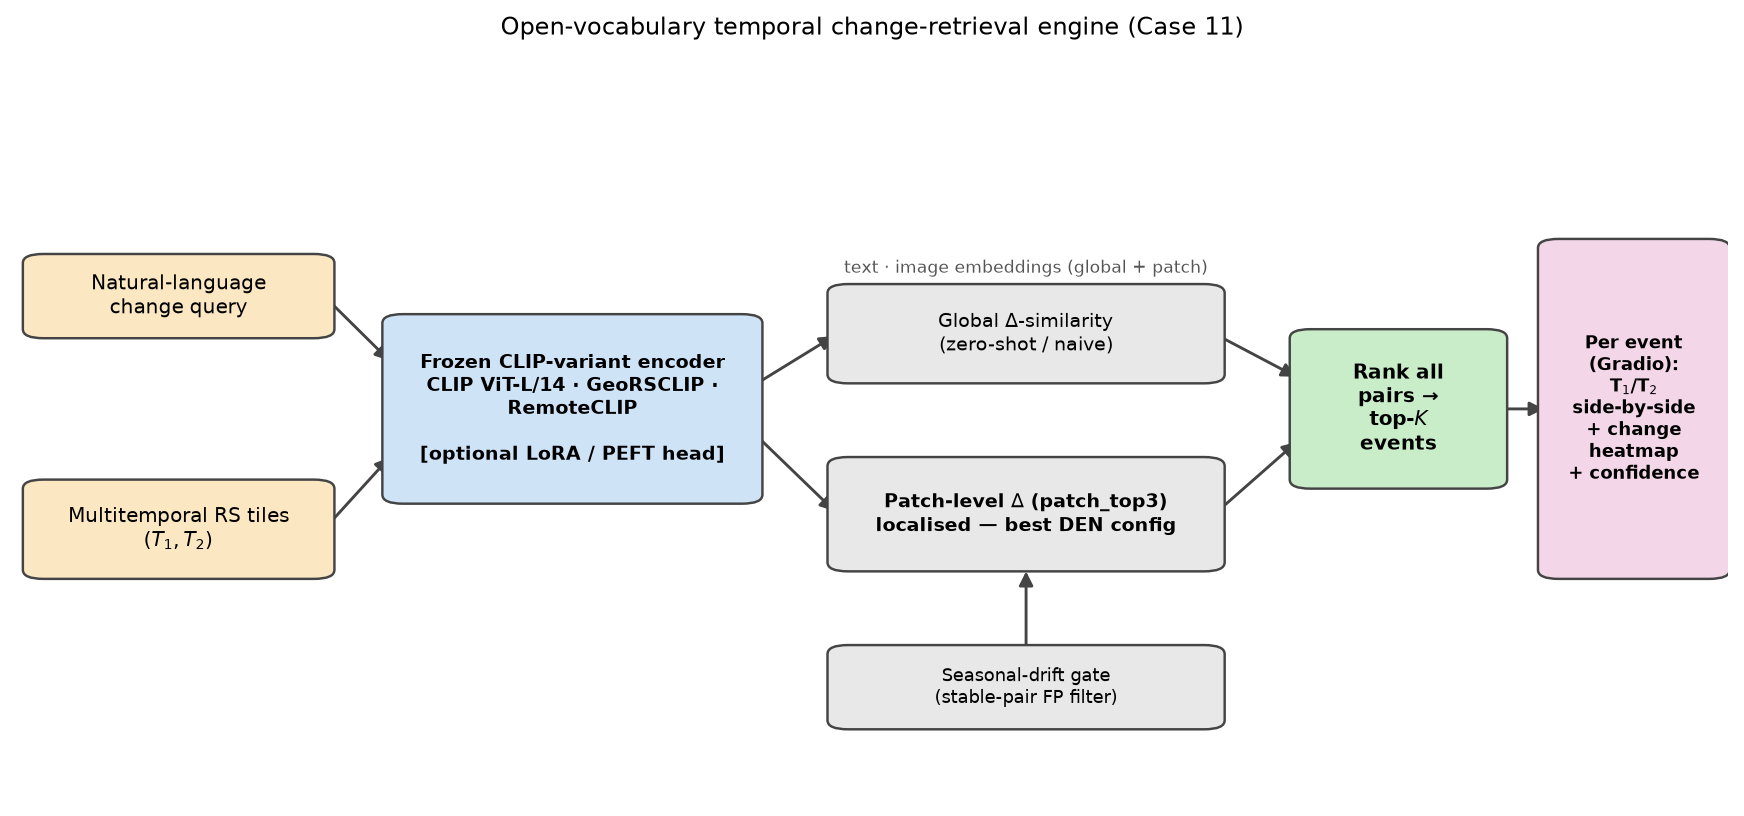
\includegraphics[width=\linewidth]{engine_pipeline.png}
    \caption{Open-vocabulary temporal change-retrieval engine. A frozen CLIP-variant encoder
    (CLIP ViT-L/14, GeoRSCLIP, or RemoteCLIP; optionally with a light LoRA/PEFT head) embeds the
    text query and both timesteps; a pair is scored by global $\Delta$-similarity or by the localised
    \texttt{patch\_top3} change score (the best Dynamic EarthNet configuration); pairs are ranked into
    the top-$K$ change events, each surfaced in the Gradio app as a $T_1/T_2$ side-by-side with a
    query-conditioned change heatmap and a confidence score. A seasonal-drift gate filters
    stable-pair false positives.}
    \label{fig:engine-pipeline}
\end{figure}

\paragraph{Dataset-agnostic core.}
A structural \texttt{TemporalDataset} protocol
(\texttt{src/datasets/base.py}) defines the only contract downstream code
depends on (list locations and pairs, load images, load metadata, derive a
\texttt{PairLabel} ground truth). A registry maps a dataset name to a factory;
the DEN factory auto-detects the on-disk layout. Concrete loaders span three
datasets and their formats and temporal axes: \texttt{DENDataset} (raster
\texttt{.tif}, monthly) and \texttt{DENNpyDataset} (DynNet preprocessed
\texttt{.npy}, 24-month) for Dynamic EarthNet; for QFabric,
\texttt{TEOChatlasQFabricDataset} (polygon-centred \texttt{.tif} crops carrying
the real RQA2 change-type labels --- the variant benchmarked in
Sections~\ref{sec:qfabric}--\ref{sec:qfabricpeft}), a RQA5 status-transition
sibling, and an EVER-Z parquet images-only loader for qualitative use; and
\texttt{LevirCCDataset} for LEVIR-CC (paired PNGs with human change captions).
Adding a dataset or encoder means adding files, never editing the shared
pipeline --- the abstraction is enforced by the protocol.

\paragraph{Encoders.}
An \texttt{ImageTextEncoder} protocol (\texttt{src/encoders/base.py}) with three
implementations: \texttt{clip\_vitl14} (HuggingFace CLIP, 768-d),
\texttt{georsclip} (\texttt{open\_clip} ViT-B/32 + RS5M checkpoint, 512-d), and
\texttt{remoteclip} (\texttt{open\_clip} ViT-L/14 + RemoteCLIP checkpoint,
768-d). The embedding dimension drives cache and index sizing automatically.

\paragraph{PEFT training.}
Only the \texttt{ProjectionHead} adapter trains; the backbones stay frozen.
Supervision is DEN's weak caption derived from its LULC labels
(e.g. ``agriculture replaced by wetlands'', ``stable forest
land cover''). The loss is a masked symmetric InfoNCE: pairs
sharing an identical caption are treated as mutual positives, which avoids the
false-negative problem of plain diagonal InfoNCE (DEN captions repeat heavily).

\paragraph{Benchmark.}
Evaluation is label-grounded: a fixed query set, where each query maps to a
relevance rule over the derived \texttt{PairLabel} (dominant $T_1$/$T_2$ class,
stability). Metrics are per-query and macro Recall@$K$, mAP, and a
seasonal-drift figure (the fraction of non-relevant top-$K$ retrievals
that involve snow/ice --- i.e. seasonal events wrongly returned for
permanent-change queries). A snapshot of the resulting Gradio search engine is
shown in Figure~\ref{fig:app}.

\begin{figure}[H]
    \centering
    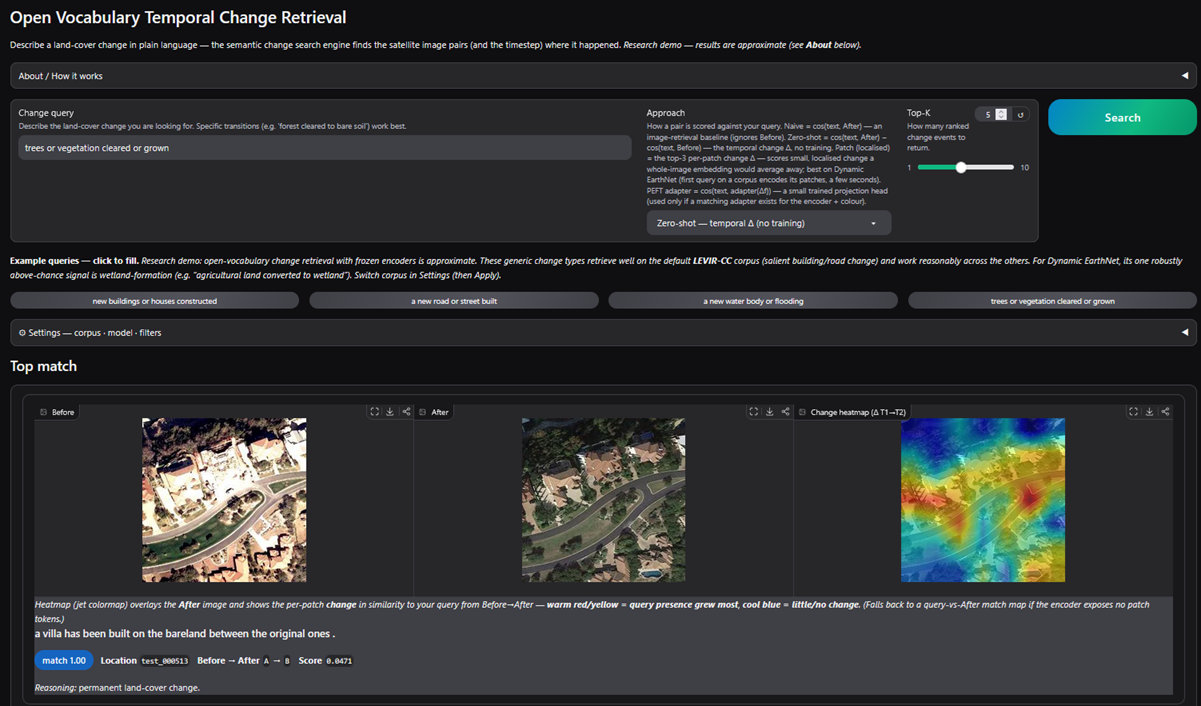
\includegraphics[width=\linewidth]{app_screenshot.png}
    \caption{The Gradio Semantic Change Search Engine: a text query returns a
    ranked list of change events, each with the $T_1$/$T_2$ pair, a localisation
    heatmap, a confidence score, and a seasonal-vs-permanent note.}
    \label{fig:app}
\end{figure}


\section{Engineering: scaffold repair and additions}
\label{sec:fixes}

The starting code base was a scaffold whose core was broken or disconnected:
the text encoder crashed, the app performed single-image retrieval rather than
change retrieval, evaluation was a synthetic identity hack, the training loop
was non-functional, two encoders were absent or mis-loading, and no data was on
disk. Table~\ref{tab:fixes} summarises the correctness fixes and additions that
were required before any experiment could run.

\begin{table}[H]
    \centering
    \caption{Key fixes and additions over the supplied scaffold.}
    \label{tab:fixes}
    \begin{tabular}{p{2.6cm}p{5.2cm}p{5.2cm}}
        \toprule
        \textbf{Area} & \textbf{Problem in scaffold} & \textbf{Resolution} \\
        \midrule
        Text encoder & \texttt{.last\_hidden\_state} on a \texttt{get\_text\_features} tensor $\rightarrow$ crash; CPU-pinned & Use \texttt{get\_text\_features} directly; device-aware (CUDA default) \\
        App & Indexed single images; returned the first two timepoints; change/adapter code unused & Rewired to real change retrieval (\texttt{ChangeRetriever}), top-$K$ events, selectors \\
        Evaluation & Identity-diagonal on synthetic random data & Label-grounded benchmark (Recall@$K$, mAP, drift) \\
        Training & Broken loop (list-of-batches, ignored shuffle, unused loss), synthetic data & Rewritten: masked symmetric InfoNCE on DEN weak captions \\
        Encoders & GeoRSCLIP a mis-loading stub; RemoteCLIP absent & Shared \texttt{open\_clip}+HF base; both implemented, registered \\
        Data & None on disk; loader assumed the wrong layout & Format-sniffing downloader; \texttt{DENNpyDataset}; synthetic fixture \\
        Robustness & Windows cp1252 crashes on non-ASCII prints & ASCII-safe console output \\
        \bottomrule
    \end{tabular}
\end{table}


\section{Retrieval approaches}
\label{sec:approaches}

Three approaches are compared end-to-end. Let $t$ be the $L_2$-normalised query
embedding and $f_{T_1}, f_{T_2}$ the $L_2$-normalised image embeddings of the
two timesteps. The scores are:

\begin{align}
    s_{\text{naive}}     &= \cos\!\big(t,\, f_{T_2}\big) && \text{(image-retrieval lower bound; no training)} \\
    s_{\text{zero\_shot}} &= \cos\!\big(t,\, f_{T_2}\big) - \cos\!\big(t,\, f_{T_1}\big) && \text{($\Delta$-similarity; no training)} \\
    s_{\text{peft}}      &= \cos\!\big(t,\, g(\Delta f)\big) && \text{($g$ = \texttt{ProjectionHead} adapter, $\sim$0.5\,M params)}
\end{align}

The naive baseline ignores the temporal dimension entirely (it scores the
``after'' image against the query). The zero-shot score measures whether the
query becomes more present from $T_1$ to $T_2$. The PEFT score passes a
change feature through a small learned adapter $g$ trained on weak captions.

\paragraph{Change-feature mode.}
The adapter consumes a change feature built from the pair embeddings, in one of
two modes (\texttt{src/features.py}): \texttt{difference}
($\Delta f = f_{T_2} - f_{T_1}$, dimension $D$) or \texttt{concatenate}
($[f_{T_1} ; f_{T_2}]$, dimension $2D$, which keeps both endpoints). Unless
otherwise stated all results use \texttt{difference}; the two modes are compared
in Section~\ref{sec:concat}.


\section{Data and encoders}
\label{sec:data}

\paragraph{Dynamic EarthNet (primary).}
The candidate DEN sources were assessed; the $\sim$525\,GB raw TUM mirror was
excluded in favour of the $\sim$7\,GB gdown preprocessed subset. A discovery
during integration: the downloaded archive (named \texttt{den\_5aoi.tar.gz}) is
in fact a ZIP, and its contents are the DynNet preprocessed
format --- per-AOI daily RGB JPEGs ($\approx$730 frames) plus
\texttt{labels/<AOI>.npy} of shape $(24, 1024, 1024)$ monthly LULC, with a
\texttt{split.json} (55 train / 10 val / 10 test AOIs). This differs from the
raster layout the original loader assumed, so we added \texttt{DENNpyDataset},
made the extractor sniff the real format, and made the registry auto-detect the
layout. The 24 monthly label maps form the change timeline; each month is mapped
to a representative daily RGB frame. These preprocessed label maps were
cross-validated against the official torchgeo Dynamic EarthNet raster masks
(\texttt{torchgeo/dynamic\_earthnet}): on the AOI tiles present in both releases
(3 AOIs, 75.5\,M valid pixels) the per-pixel class agreement is 99.9999\%,
confirming the preprocessing preserves the published ground truth. The official
release withholds the held-out test labels, which the preprocessed subset
retains. A deterministic synthetic DEN fixture
(\texttt{scripts/make\_den\_fixture.py}) reproduces the on-disk layout and an
engineered label signal (urban growth, deforestation, seasonal snow-melt, stable
negatives), so the full pipeline is testable in seconds with no network.

DEN also provides an on-disk near-infrared band (\texttt{\_infra.jpeg}, one
grayscale frame per daily timestep), which we expose through three
colour modes: \texttt{rgb} (standard 3-channel), \texttt{nrg}
(NIR-Red-Green false-colour) and \texttt{ndvi} (single-band NDVI replicated
across three channels). The working corpus is 605 bimonthly pairs on the train
split, and 110 pairs each on val and test.

\paragraph{QFabric (secondary).}
QFabric is wired as a second dataset to validate the dataset-agnostic design,
using the polygon-centred crops from \texttt{jirvin16/TEOChatlas} with the
real QFabric change-type labels (the TEOChatlas RQA2 answers; 27{,}879
labelled crops). It contributes a different taxonomy (6 construction
change-types), sensor, and crop scale.

\paragraph{LEVIR-CC (third dataset, human change captions).}
LEVIR-CC (Liu et al., 2022) adds a third dataset with a fundamentally different
label source: 10{,}077 bi-temporal building-change pairs ($256\times256$,
0.5\,m), each annotated with five human-written change captions and a binary
change flag (5{,}038 changed / 5{,}039 unchanged). We parse the captions into
open-vocabulary change tags (building, road, demolition, vegetation, water) so
that free-text queries map directly to caption-grounded relevance, exposed
through the same protocol (\texttt{src/datasets/levir\_cc.py}). It tests the
engine on salient, well-described change described in genuine human language,
complementing DEN's subtle spectral transitions and QFabric's categorical types.
The five caption tags include vegetation and water, broadening the original
three-query (building/road/demolition) evaluation to five.

\paragraph{LEVIR-MCI (localisation masks on the LEVIR pairs).}
LEVIR-MCI (Liu et al., 2024) is a strict superset of LEVIR-CC --- the same
10{,}077 pairs and captions, plus a pixel-level building/road change mask per
pair. We store it once and serve both \texttt{levir\_cc} and \texttt{levir\_mci}
from it (\texttt{src/datasets/levir\_mci.py}); the masks make the change-heatmap
deliverable quantitatively measurable (Section~\ref{sec:localization}).

\paragraph{SECOND-CC (fourth dataset, open-vocabulary breadth + semantic masks).}
SECOND-CC (Robust Change Captioning in Remote Sensing, 2025) pairs 6{,}041
bi-temporal scenes with 30{,}205 human change captions \emph{and} six-class
SECOND semantic maps for both phases (ground, tree, low-vegetation, water,
building, playground). It is the breadth counterpart to LEVIR-CC, whose change is
almost entirely building/road: SECOND-CC's captions span a far wider land-cover
vocabulary, and its per-phase semantic maps give both retrieval relevance
(caption tags) and localisation ground truth (per-class and directed-transition
change masks), through the same protocol (\texttt{src/datasets/second\_cc.py}).

\paragraph{Encoders.}
Table~\ref{tab:encoders} lists the three frozen CLIP-variant encoders. All
embeddings are $L_2$-normalised; the dimension automatically drives cache and
index sizing.

\begin{table}[H]
    \centering
    \caption{The three frozen vision-language encoders.}
    \label{tab:encoders}
    \begin{tabular}{lllr}
        \toprule
        \textbf{Encoder} & \textbf{Backbone} & \textbf{Pre-training} & \textbf{Dim} \\
        \midrule
        \texttt{clip\_vitl14} & ViT-L/14 (HuggingFace CLIP)        & general (CLIP)       & 768 \\
        \texttt{georsclip}    & ViT-B/32 (\texttt{open\_clip})     & RS5M (remote sensing) & 512 \\
        \texttt{remoteclip}   & ViT-L/14 (\texttt{open\_clip})     & RemoteCLIP            & 768 \\
        \bottomrule
    \end{tabular}
\end{table}


\section{Experiments and results}
\label{sec:results}

All headline experiments use real Dynamic EarthNet. The fast test suite (mock
encoders, synthetic fixture, no network) passes 234 tests (full suite
250: 249 passed, 1 skipped) and covers the embeddings cache and round-trip,
retrieval (naive/zero\_shot/peft), benchmark metrics, PEFT training
(loss decreases, save/load), the encoder protocol/registry, and the app's
\texttt{query()} path (real fixture tiles + heatmap + seasonal note). The
subsections below report the quantitative results. All DEN numbers are
audited in Section~\ref{sec:audit} (random baselines, FDR, cross-validation),
which is the authoritative reading --- the per-split tables below are raw
measurements, not the generalisation verdict.

\subsection{Training-set fit (train split, 605 pairs, RGB)}
\label{sec:indist}

Using the \texttt{difference} change feature, Table~\ref{tab:indist} reports mAP
and macro Recall@10 on the train split. This should be read as a sanity check, not
a result: the PEFT column is the adapter evaluated on the very pairs it was
trained on, so it measures memorisation capacity, not retrieval. The
generalisation verdict is the held-out cross-validation in Section~\ref{sec:audit}.

\begin{table}[H]
    \centering
    \caption{Training-set fit (train split, 605 pairs, RGB, \texttt{difference}) ---
    PEFT scored on its own training pairs (memorisation), not a held-out result.}
    \label{tab:indist}
    \begin{tabular}{lcccc}
        \toprule
        \textbf{Encoder} & \textbf{naive} & \textbf{zero-shot} & \textbf{PEFT} & \textbf{PEFT R@10} \\
        \midrule
        CLIP ViT-L/14 (768-d)       & 0.031 & 0.043 & \textbf{0.420} & 0.36 \\
        GeoRSCLIP ViT-B/32 (512-d)  & 0.027 & 0.040 & \textbf{0.335} & 0.26 \\
        RemoteCLIP ViT-L/14 (768-d) & 0.024 & 0.057 & \textbf{0.352} & 0.30 \\
        \bottomrule
    \end{tabular}
\end{table}

Three observations follow. First, zero-shot is near chance: $\Delta$-similarity
beats the naive image baseline only marginally, and neither separates change
types, because CLIP and GeoRSCLIP embed scene appearance, not directional
land-cover transition, so differencing two normalised global embeddings discards
the localised change signal. Second, PEFT only fits the training pairs --- the
$\sim$8--10$\times$ lift confirms the adapter has the capacity to memorise the 55
training AOIs, but it says nothing about retrieval skill until evaluated
out-of-distribution (Section~\ref{sec:crosssplit}), where it collapses; on
QFabric the same train-fit reaches mAP 0.998, which is unmistakably
memorisation. Third,
the train-fit ranking reflects memorisation capacity, not generalisation: CLIP
ViT-L/14 (0.420) $>$ RemoteCLIP (0.352) $>$ GeoRSCLIP (0.335), the larger
backbone fitting hardest, but this ordering reverses on held-out data (GeoRSCLIP
leads, Section~\ref{sec:nir}). On zero-shot, RS pre-training already helps
in-sample (RemoteCLIP 0.057 best).

\begin{figure}[H]
    \centering
    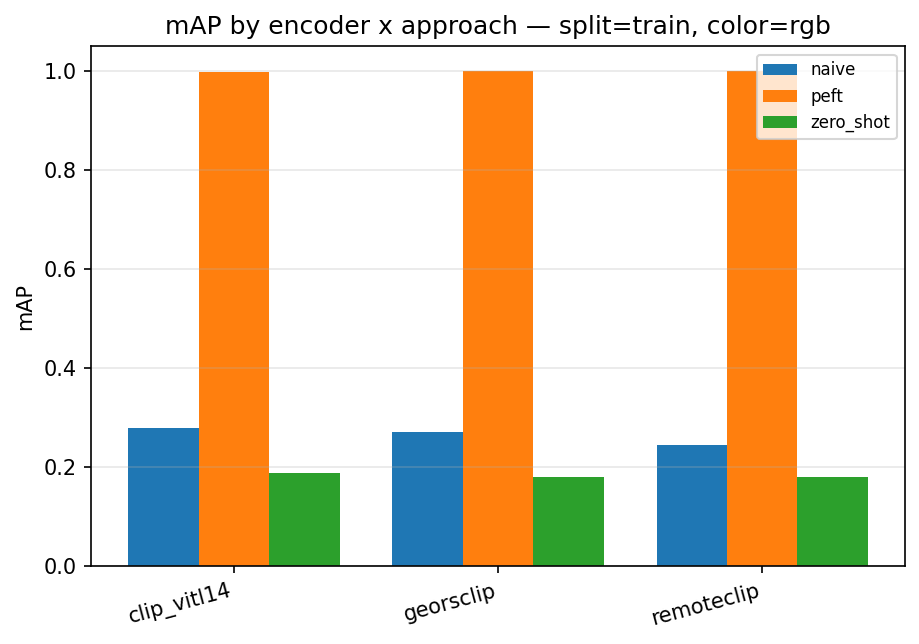
\includegraphics[width=0.8\linewidth]{map_bars__train__rgb.png}
    \caption{mAP by encoder $\times$ approach on the train split (RGB).}
    \label{fig:mapbars_train}
\end{figure}

\begin{figure}[H]
    \centering
    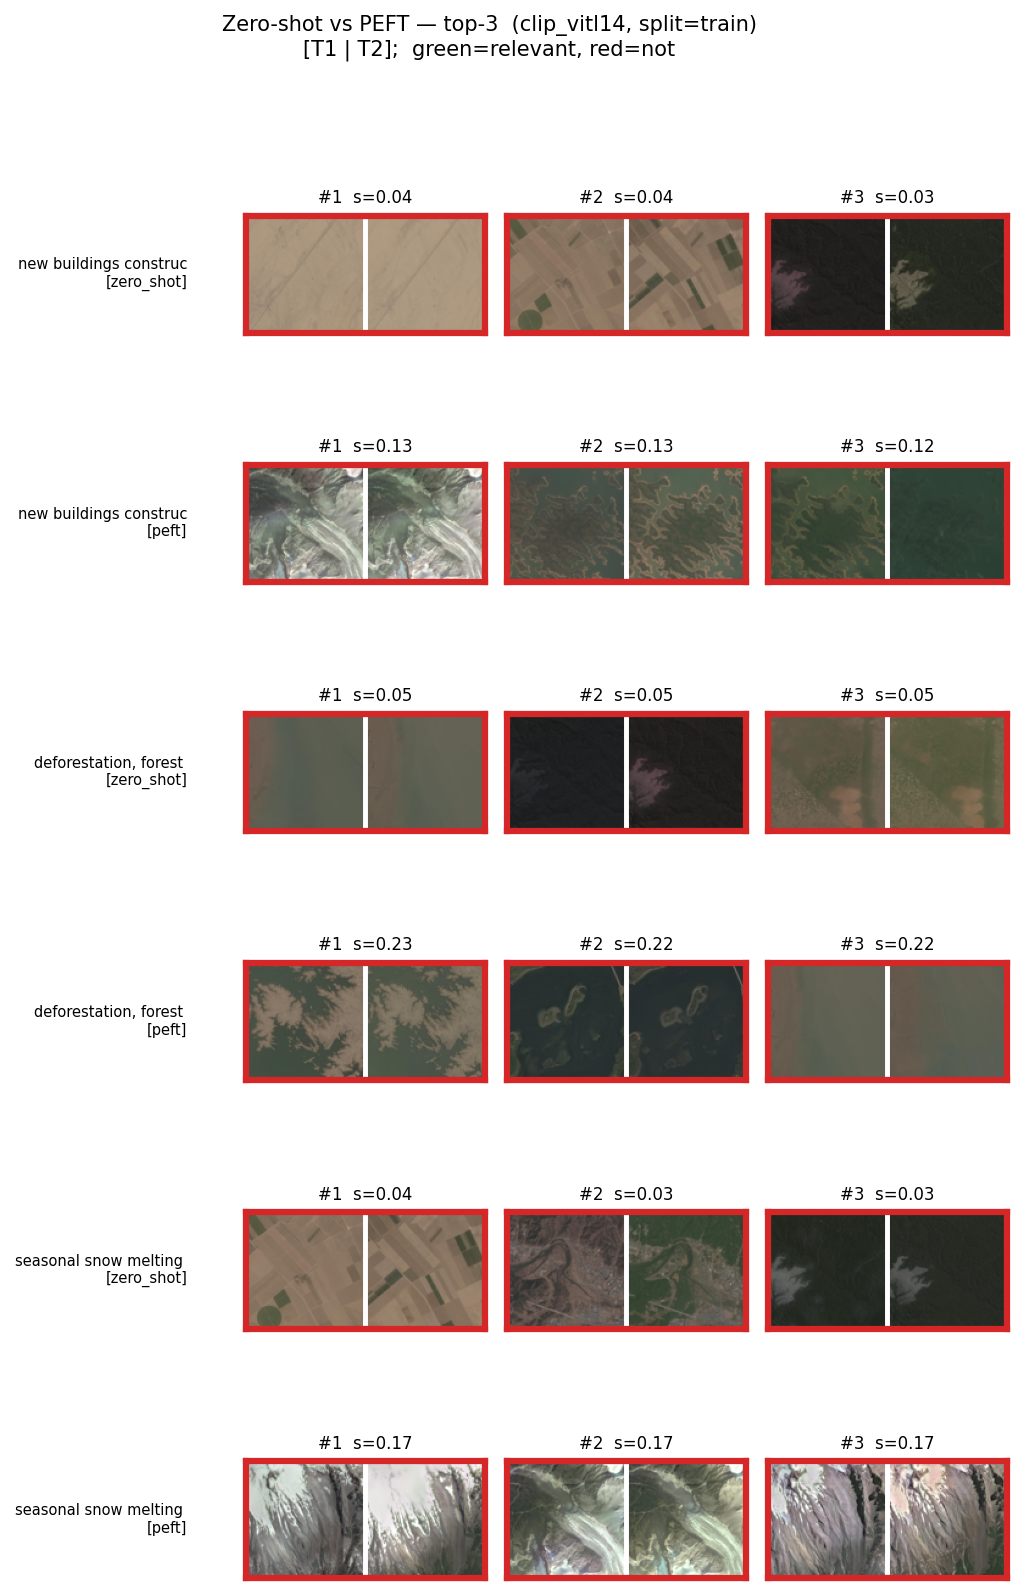
\includegraphics[width=0.9\linewidth]{zeroshot_vs_peft__clip_vitl14__train.png}
    \caption{Qualitative zero-shot vs PEFT (CLIP, train): top-3 retrievals per
    query, $[T_1 \mid T_2]$, green = relevant. The adapter sharpens scores, but
    the gain is concentrated on the classes its weak captions cover.}
    \label{fig:zsvspeft}
\end{figure}

\subsection{Cross-split generalisation}
\label{sec:crosssplit}

The adapter is trained on the train split and evaluated on train/val/test
(RGB, \texttt{difference}). Table~\ref{tab:crosssplit} reports mAP per split.

\begin{table}[H]
    \centering
    \caption{Cross-split mAP (adapter trained on train; RGB, \texttt{difference}).}
    \label{tab:crosssplit}
    \begin{tabular}{llccc}
        \toprule
        \textbf{Encoder} & \textbf{approach} & \textbf{train} & \textbf{val} & \textbf{test} \\
        \midrule
        CLIP ViT-L/14       & naive     & 0.031 & 0.053 & 0.046 \\
        CLIP ViT-L/14       & zero-shot & 0.043 & 0.051 & 0.043 \\
        CLIP ViT-L/14       & \textbf{PEFT} & \textbf{0.420} & \textbf{0.042} & \textbf{0.040} \\
        GeoRSCLIP ViT-B/32  & naive     & 0.027 & 0.030 & 0.061 \\
        GeoRSCLIP ViT-B/32  & zero-shot & 0.040 & 0.036 & 0.299 \\
        GeoRSCLIP ViT-B/32  & \textbf{PEFT} & \textbf{0.335} & \textbf{0.087} & \textbf{0.041} \\
        RemoteCLIP ViT-L/14 & naive     & 0.024 & 0.029 & 0.121 \\
        RemoteCLIP ViT-L/14 & zero-shot & 0.057 & 0.025 & 0.050 \\
        RemoteCLIP ViT-L/14 & \textbf{PEFT} & \textbf{0.352} & \textbf{0.028} & \textbf{0.103} \\
        \bottomrule
    \end{tabular}
\end{table}

\noindent On the evaluation basis, mAP is
macro-averaged only over queries with $\geq$1 positive in that corpus
(zero-positive queries are dropped), so the evaluable query set differs per
split. The headline GeoRSCLIP NRG test result (0.426, Section~\ref{sec:nir})
rests on 3 evaluable wetland queries / 15 positives among 110 pairs --- a small
basis that does not survive cross-validation (Section~\ref{sec:audit}:
full-corpus 0.037, 5-fold 0.100); the bold train column is moreover the
adapter scored on its own training pairs, so only the val/test columns are a
held-out measurement.

\medskip

\noindent The key finding is that PEFT overfits to train AOIs. The adapter
memorises spatial statistics of the 55 training locations rather than learning
generalised change semantics; on unseen val and test AOIs it is equal to or
worse than zero-shot. GeoRSCLIP zero-shot reaches 0.299 mAP on the test split
without any training, suggesting the test AOIs contain transitions that
RS-domain features represent more discriminatively than train. The
train-spike-then-collapse signature is plotted in Figure~\ref{fig:crosssplit}.

\begin{figure}[H]
    \centering
    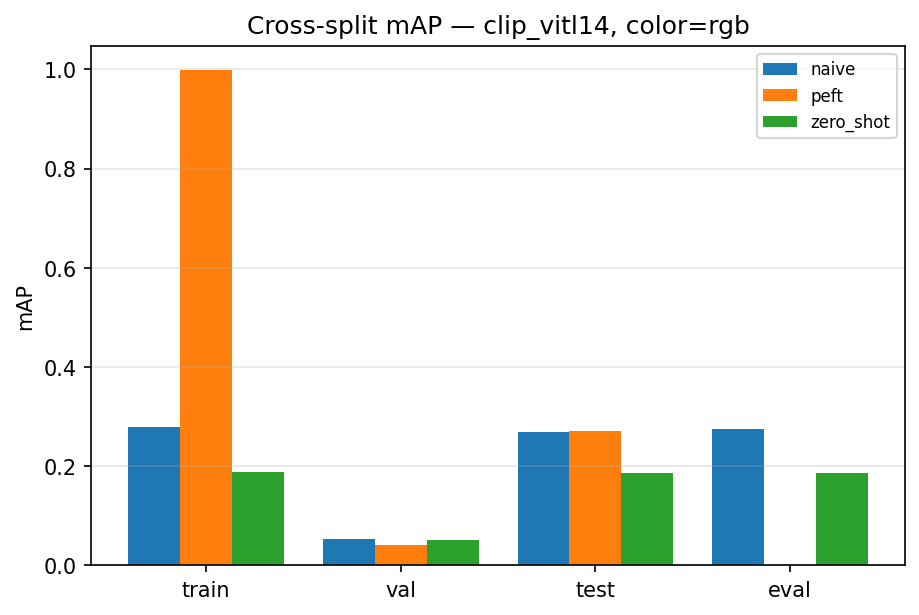
\includegraphics[width=0.8\linewidth]{cross_split__clip_vitl14__rgb.png}
    \caption{Cross-split mAP for CLIP ViT-L/14 (RGB): the PEFT train spike
    collapses on held-out val/test.}
    \label{fig:crosssplit}
\end{figure}

\subsection{NIR false-colour ablation}
\label{sec:nir}

Three colour modes are compared (zero-shot mAP, all three splits) in
Table~\ref{tab:nir}.

\begin{table}[H]
    \centering
    \caption{Colour-mode ablation (zero-shot mAP). NRG is the best colour mode on
    held-out test for every encoder. Best test per encoder in bold.}
    \label{tab:nir}
    \begin{tabular}{llccc}
        \toprule
        \textbf{Encoder} & \textbf{color} & \textbf{train} & \textbf{val} & \textbf{test} \\
        \midrule
        CLIP ViT-L/14 & RGB  & 0.043 & 0.051 & 0.043 \\
        CLIP ViT-L/14 & NRG  & 0.033 & 0.066 & \textbf{0.104} \\
        CLIP ViT-L/14 & NDVI & 0.032 & 0.045 & 0.064 \\
        GeoRSCLIP     & RGB  & 0.040 & 0.036 & 0.299 \\
        GeoRSCLIP     & \textbf{NRG}  & 0.025 & 0.030 & \textbf{0.426} \\
        GeoRSCLIP     & NDVI & 0.028 & 0.065 & 0.216 \\
        RemoteCLIP    & RGB  & 0.057 & 0.025 & 0.050 \\
        RemoteCLIP    & NRG  & 0.023 & 0.047 & \textbf{0.129} \\
        RemoteCLIP    & NDVI & 0.022 & 0.048 & 0.055 \\
        \bottomrule
    \end{tabular}
\end{table}

NRG hurts on train ($-0.010$ to $-0.034$) but substantially helps on test
($+0.061$ CLIP, $+0.127$ GeoRSCLIP, $+0.079$ RemoteCLIP). NDVI usually lands
between NRG and RGB (though for GeoRSCLIP its single-channel collapse drops it
below even RGB on test, 0.216 vs 0.299): NDVI provides some NIR signal but
collapses all spectral texture into a single channel replicated across R/G/B, so
the RS-pretrained encoders cannot exploit the inter-channel colour contrasts that
NRG preserves. RemoteCLIP NRG
(test 0.129) improves over RGB (0.050) but lags GeoRSCLIP NRG (single-split 0.426):
GeoRSCLIP's RS5M pre-training gives it a stronger prior for the NIR-Green
spectral contrast characteristic of vegetation transitions.

GeoRSCLIP + NRG zero-shot is the best configuration on this test split
(0.426), but this number is not robust: under 5-fold AOI
cross-validation it falls to $0.100 \pm 0.139$ (Section~\ref{sec:audit}); the
110-pair test split is a high-wetland ``lucky fold'' (CV folds span
0.032--0.348). NRG remaining the best colour mode for every encoder, and the
encoder ordering (GeoRSCLIP $\gg$ CLIP $\approx$ RemoteCLIP), both hold, but the
absolute 0.426 should not be read as the generalisation result.

\begin{figure}[H]
    \centering
    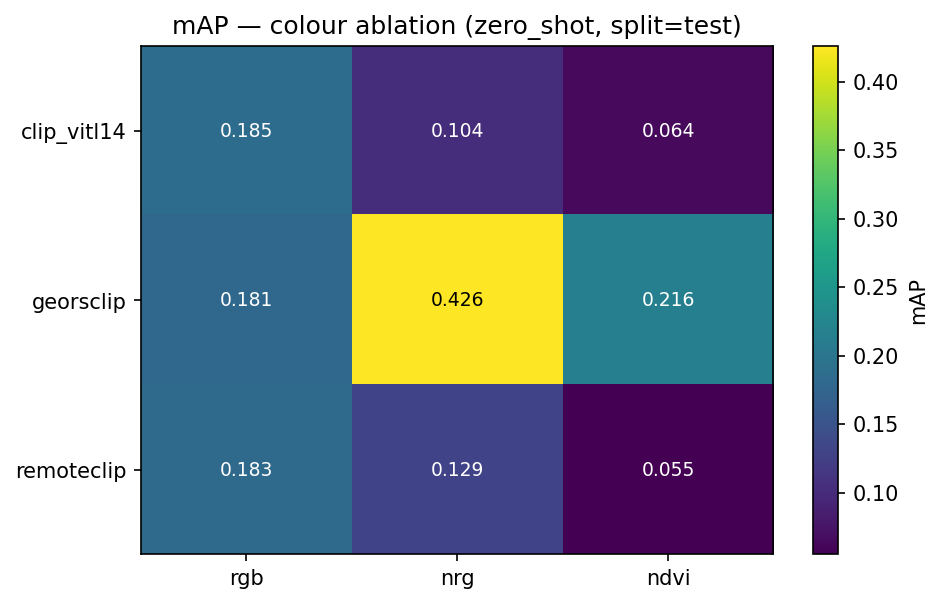
\includegraphics[width=0.8\linewidth]{color_ablation__zero_shot__test.png}
    \caption{Colour-mode ablation (zero-shot, test split): NRG dominates,
    most strongly for GeoRSCLIP.}
    \label{fig:colorablation}
\end{figure}

\subsection{LoRA adapter --- visual-encoder fine-tuning}
\label{sec:lora}

LoRA applied to GeoRSCLIP's ViT-B/32 visual encoder targets the FFN projections
\texttt{c\_fc} and \texttt{c\_proj} in each ResBlock: 368{,}640 trainable params
out of 88M (0.42\%). The attention output projection \texttt{out\_proj} is
deliberately not adapted --- open\_clip's attention is an
\texttt{nn.MultiheadAttention} whose forward reads \texttt{out\_proj.weight}
directly (via \texttt{F.multi\_head\_attention\_forward}) and never calls
\texttt{out\_proj.forward}, so a PEFT LoRA wrapper there receives no gradient and
is a silent no-op. Training is online (no pre-cached
embeddings; images loaded on the fly) using the same masked symmetric InfoNCE
loss as the ProjectionHead (mean log-prob over each row's same-caption positive
set). Table~\ref{tab:lora} compares frozen
zero-shot against LoRA-adapted zero-shot (GeoRSCLIP + NRG, rank=4, $\alpha$=8,
20 epochs).

\begin{table}[H]
    \centering
    \caption{LoRA (GeoRSCLIP + NRG) vs frozen zero-shot. LoRA fits train and
    matches val but collapses on the held-out test split. Best per row in bold.}
    \label{tab:lora}
    \begin{tabular}{lcc}
        \toprule
        \textbf{split} & \textbf{zero\_shot (frozen)} & \textbf{LoRA zero\_shot} \\
        \midrule
        train & 0.025 & \textbf{0.153} \\
        val   & 0.030 & \textbf{0.034} \\
        test  & \textbf{0.426} & 0.071 \\
        \bottomrule
    \end{tabular}
\end{table}

LoRA now fits the train split ($0.025 \rightarrow 0.153$) but collapses
out-of-distribution ($0.426 \rightarrow 0.071$ on test) --- a textbook overfit.
That test $0.071$ is numerically just above ProjectionHead PEFT's RGB test
($0.041$), but the comparison is cross-colour-mode and both sit at or below the
DEN-test random floor ($\approx 0.083$) --- neither learned adapter beats chance
on held-out AOIs. To check whether a
different capacity changes this, we swept rank and epochs
(Table~\ref{tab:lorasweep}; \texttt{scripts/lora\_sweep.py}, in-memory, no
cache/model clobber).

\begin{table}[H]
    \centering
    \caption{LoRA rank/epoch sweep (GeoRSCLIP + NRG, zero\_shot mAP). Every
    configuration fits train yet collapses on test --- no capacity sweet spot.}
    \label{tab:lorasweep}
    \begin{tabular}{ccccc}
        \toprule
        \textbf{rank} & \textbf{$\alpha$} & \textbf{epochs} & \textbf{train} & \textbf{test} \\
        \midrule
        4  & 8  & 20 & 0.153 & 0.071 \\
        8  & 16 & 20 & 0.168 & 0.070 \\
        16 & 32 & 20 & 0.135 & 0.058 \\
        8  & 16 & 40 & 0.146 & 0.059 \\
        \bottomrule
    \end{tabular}
\end{table}

There is no capacity sweet spot: every rank/epoch setting fits the train split
(0.13--0.17, well above the frozen 0.025) yet overfits to test 0.06--0.07. More
rank or more epochs only memorise harder; the best test (0.071) still sits far
below frozen NRG zero-shot (single-split 0.426). This reinforces the project's core finding
that spectral physics (NRG false-colour) generalises while learned visual priors
only memorise --- and is sharper than the earlier reading, which was distorted by
a since-fixed LoRA loss bug and a stale-cache reuse.

\begin{figure}[H]
    \centering
    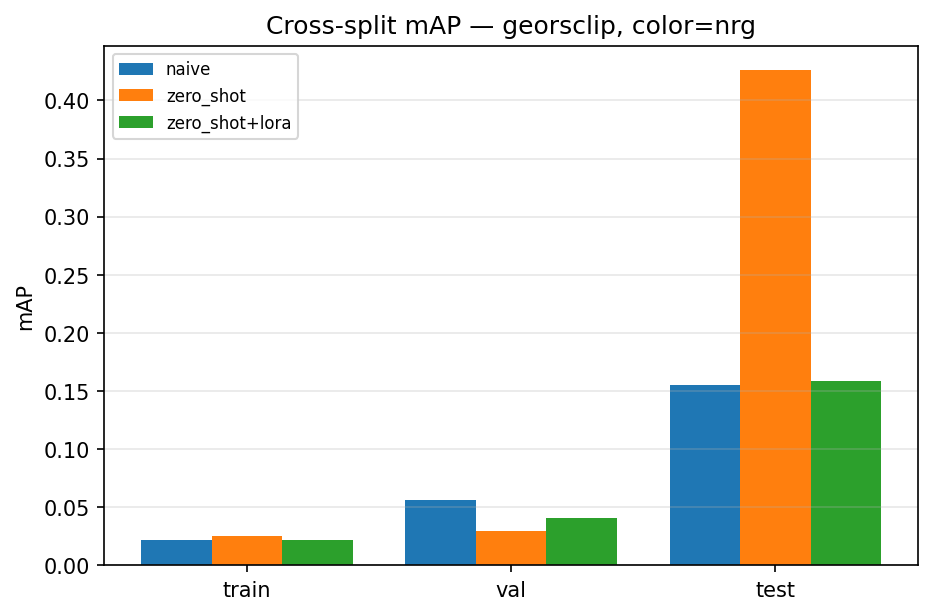
\includegraphics[width=0.8\linewidth]{cross_split__georsclip__nrg.png}
    \caption{GeoRSCLIP + NRG: frozen zero-shot vs LoRA across splits.}
    \label{fig:loracross}
\end{figure}

\subsection{Statistical audit, cross-validation, and method fixes}
\label{sec:audit}

The per-split tables above are raw single-split measurements. Re-auditing them
against a Monte-Carlo random-ranking baseline (relevant set fixed, ranking
shuffled), with Benjamini--Hochberg FDR correction and leave-one-AOI-out
cross-validation, materially changes the reading. Two metric caveats first:
Recall@$K$ on QFabric is ceiling-bounded (with 480 relevant pairs, $R@10 \le
10/480 = 0.021$), so QFabric is judged by mAP only; and a random ranker scores
mAP $\approx$ prevalence (0.17 on QFabric-TEO, 0.08 on DEN-test), so mAP must be
read against that floor, not against 0.

\medskip\noindent The 0.426 headline is a lucky fold. Merging the cached
train+val+test embeddings (all 75 AOIs, 825 pairs --- no re-encoding) and
re-evaluating on the full corpus and under 5-fold AOI cross-validation collapses
every test-split number (Table~\ref{tab:cv}). GeoRSCLIP+NRG goes from 0.426 to a
full-corpus 0.037 / cross-validated $0.100 \pm 0.139$ (folds span 0.032--0.348;
the 110-pair test split coincided with the easy high-wetland fold). Leakage-free
cross-validated PEFT on GeoRSCLIP+NRG ($0.196 \pm 0.049$, fraction relevance)
overlaps frozen zero-shot ($0.139 \pm 0.024$) within fold variance --- neither a
collapse nor a gain --- confirming the high in-distribution PEFT figures
($0.42$--$0.998$) were memorisation, not generalisation.

\begin{table}[H]
    \centering
    \caption{GeoRSCLIP NRG zero-shot: the test-split mAP does not survive
    cross-validation. ``S1'' = pixel-fraction relevance; ``S3'' = patch-level
    scoring (below). Random baseline $\approx$ 0.08.}
    \label{tab:cv}
    \begin{tabular}{lccc}
        \toprule
        \textbf{Evaluation} & \textbf{test split} & \textbf{full corpus} & \textbf{5-fold CV} \\
        \midrule
        dominant-flip relevance      & 0.426 & 0.037 & $0.100 \pm 0.139$ \\
        + fraction relevance (S1)    & ---   & 0.091 & $0.139 \pm 0.024$ \\
        + patch top-3 scoring (S3)   & ---   & 0.122 & $\mathbf{0.193 \pm 0.051}$ \\
        \bottomrule
    \end{tabular}
\end{table}

\noindent The weakness is not the data but the evaluation, and beyond that a method
ceiling. The labels are complete and dense (per-pixel 7-class, 24 months, all
75 AOIs). The bottleneck was the relevance rule: a pair counted as a positive
only if the dominant class of the whole $1024^2$ tile flips, which happens
for just 8.6\% of pairs (71/825), 44 of them wetland$\leftrightarrow$agriculture
--- starving every other query. Re-deriving relevance from the per-class
pixel-fraction change that the labels already contain (``S1'', $\geq$5\% of
pixels) makes 9 of 10 queries evaluable (new buildings 14 positives,
deforestation 13, soil 25, water 9 --- previously 0--3), roughly triples
full-corpus mAP, and tightens the cross-validation interval (Table~\ref{tab:cv}).
Only snow remains genuinely absent from the subset.

\medskip\noindent Even with correct dense labels, the method is the
ceiling, and a localised scorer partly fixes it (``S3''). Under fraction
relevance, global-embedding zero-shot still leaves localised change-types (new
buildings, urban expansion, water) at chance, because differencing two global
$1024^2$ embeddings dilutes a small change region. Scoring instead from
per-patch embeddings (\texttt{scripts/patch\_eval.py}: the mean of the
top-3 per-patch $\Delta$-similarities) lifts cross-validated mAP to
$0.193 \pm 0.051$ --- the best DEN configuration found --- and makes new
buildings ($q{=}0.003$) and urban expansion ($q{=}0.006$) beat random (FDR-corrected)
for the first time, with new water borderline ($q{=}0.053$) (Figure~\ref{fig:cvprogression}). Diffuse
large-area wetland change still prefers the global score, so the two are
complementary. Notably GeoRSCLIP's coarse 49-patch grid beats CLIP-L/14's finer
256-patch grid (0.193 vs 0.149): domain pre-training outweighs patch resolution.

\begin{figure}[H]
    \centering
    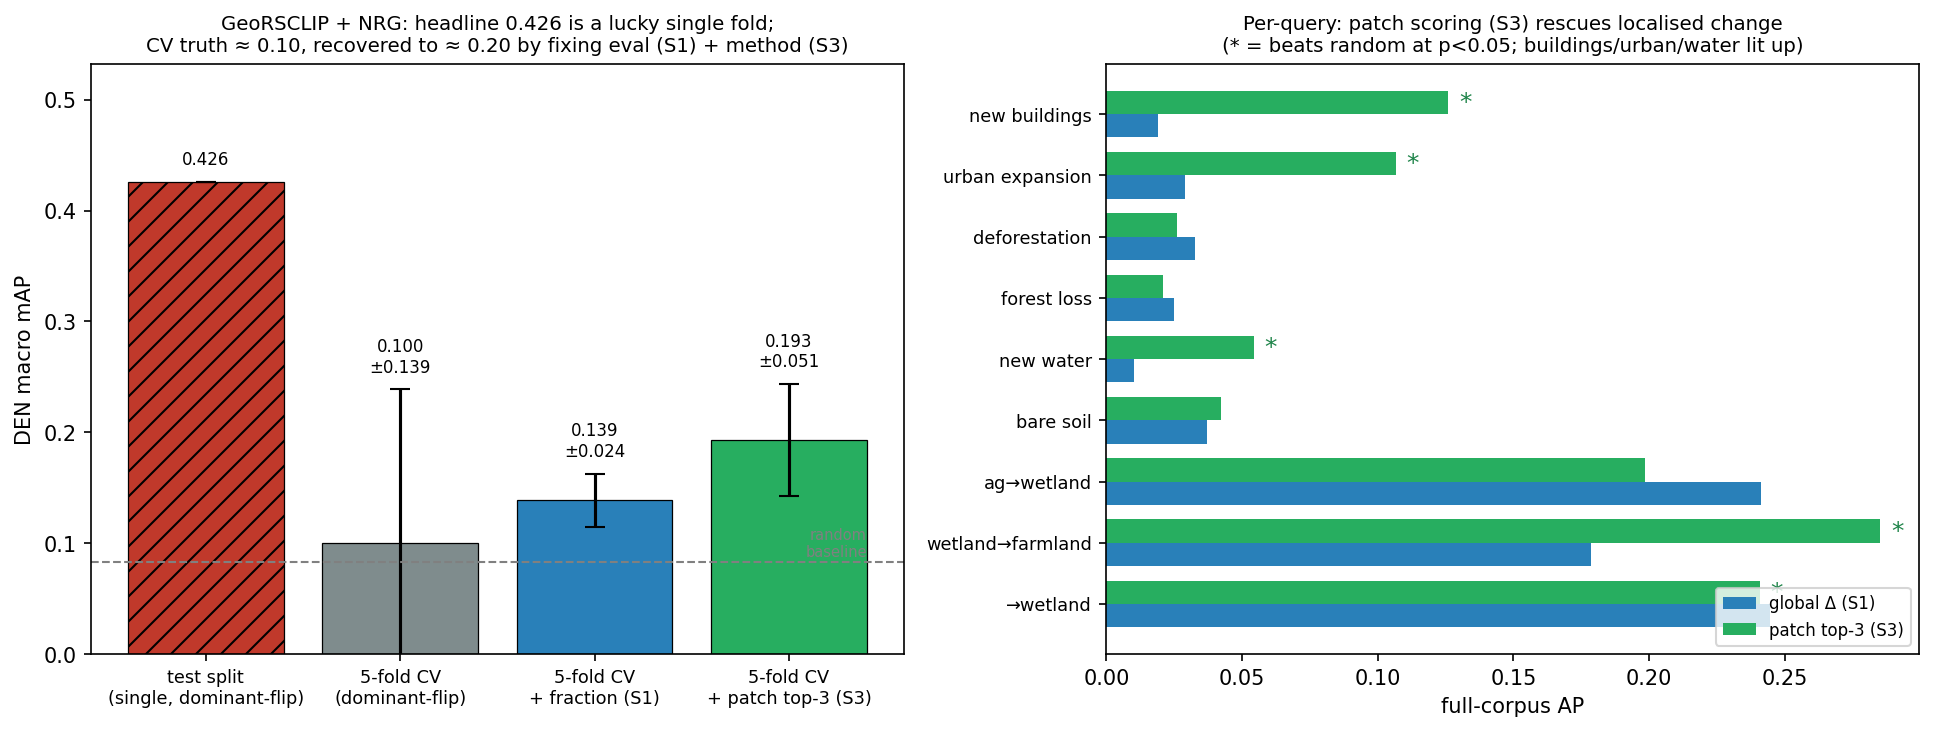
\includegraphics[width=\linewidth]{cv_progression.png}
    \caption{DEN result chain (GeoRSCLIP+NRG). Left: the 0.426 test-split
    headline collapses under cross-validation, then recovers to $\approx$0.20 by
    fixing evaluation (S1) and method (S3). Right: per-query, patch-level
    scoring (S3) rescues localised change-types (buildings/urban/water) that
    global pooling left at chance ($*$ = beats random, $p<0.05$).}
    \label{fig:cvprogression}
\end{figure}

\noindent The defensible DEN claim is therefore narrow but honest: a frozen,
RS-pre-trained encoder with NIR false-colour and localised patch scoring
retrieves construction change (new buildings, urban expansion) and large-area
wetland change above chance, with new water borderline
($\approx$0.20 cross-validated mAP); no learned adapter beats it on held-out data;
and naive single-split numbers (the 0.426) overstate this by $\sim$2$\times$.

\medskip\noindent Several cheaper in-scope refinements were tested and none
improved on patch top-3, reported here as honest negatives. Averaging the query
embedding over a prompt ensemble is a wash (0.142 cross-validated mAP); fusing the
global $\Delta$-cosine with the patch score by z-scoring and summing hurts
(0.165), the mostly-noise global signal diluting the stronger patch signal; and
two training-free change-attention variants --- query-conditioned soft-attention
over the per-patch $\Delta$ (0.137) and $3\times3$ spatial smoothing of the
$\Delta$-map (0.168) --- refine the aggregation without breaking the
$\approx$0.20 ceiling. Routing each query by its a-priori spatial geometry ---
diffuse phrasings to the global score, localised ones to patch top-3 --- scores
$0.186 \pm 0.051$ under the same cross-validation, statistically
indistinguishable from ungated patch top-3 and recovering the same four
FDR-significant queries, so query geometry is not a usable routing signal at
this encoder scale. A learned query-to-patch attention head was deliberately
not pursued, since every trained head on this data memorises the training AOIs
with no held-out gain (Section~\ref{sec:crosssplit}).

\subsection{Native 3\,m raster source --- robustness of the data-source choice}
\label{sec:nativeraster}

Section~\ref{sec:data} excluded the $\sim$525\,GB raw TUM mirror in favour of the
$\sim$7\,GB preprocessed RGB/NIR-JPEG subset. To check that this pragmatic choice
does not cost retrieval performance --- i.e.\ that the conclusions survive at full
radiometric depth --- we ran an independent replication directly on the excluded
source: the native Planet-Fusion surface-reflectance rasters
($1024\times1024\times4$ \texttt{int16}, Blue/Green/Red/NIR, 3\,m), read in-memory
from the per-zone \texttt{planet.<UTM>.zip} archives with no lossy re-encoding. The
full mirror was made tractable by cherry-picking only the UTM zones needed via
\texttt{rsync} \texttt{--include}/\texttt{--exclude} and decoding tiles straight
from the zips, yielding 23 labelled AOIs (552 bimonthly change pairs) spanning all
seven DEN land-cover classes.

The adapter (frozen CLIP ViT-L/14, \texttt{difference} change feature) was scored
under the same held-out protocol as Section~\ref{sec:audit}: a 5-seed stratified
\emph{AOI}-level hold-out (split on real cube id to prevent leakage, stratified by
dominant change class), reporting mean $\pm$ std across seeds.
Table~\ref{tab:nativeraster} reports the result.

\begin{table}[H]
    \centering
    \caption{Native 3\,m raster source (CLIP ViT-L/14, adapter, \texttt{difference};
    23 AOIs, 5-seed stratified AOI cross-validation). NIR here is the
    NIR-Red-Green false colour (matching \texttt{nrg} elsewhere).}
    \label{tab:nativeraster}
    \begin{tabular}{llc}
        \toprule
        \textbf{Configuration} & \textbf{colour} & \textbf{mAP (mean $\pm$ std)} \\
        \midrule
        Adapter                & RGB  & 0.236 $\pm$ 0.030 \\
        Adapter                & NIR (NRG)  & 0.253 $\pm$ 0.040 \\
        Adapter, class-weighted & RGB & 0.265 $\pm$ 0.029 \\
        Adapter, $2\times2$ patch tiling & RGB & 0.202 $\pm$ 0.022 \\
        \bottomrule
    \end{tabular}
\end{table}

Two readings follow, both consistent with the JPEG-subset audit. First, the native
rasters land in the \emph{same band} as the preprocessed subset under
cross-validation (cf.\ the audited CV figures in Section~\ref{sec:audit}): full
\texttt{int16} radiometric depth and the intact NIR channel buy no material
retrieval gain over the $\sim$7\,GB RGB/NIR-JPEG subset, so the data-source choice
in Section~\ref{sec:data} is vindicated --- the bottleneck is the frozen
web-pretrained features and the small labelled AOI set, not imagery compression.
Second, no full-tile configuration is statistically separable from another: RGB
($0.236\pm0.030$), NRG ($0.253\pm0.040$) and per-class loss weighting
($0.265\pm0.029$) all overlap within one standard deviation, and the $+0.017$
NRG-over-RGB margin sits well inside that noise --- the same null result as
Section~\ref{sec:nir}, where the large single-split NRG lift collapses under
cross-validation, confirming it is a fold artefact rather than a spectral effect.
Only $2\times2$ patch tiling separates, and downward ($0.202\pm0.022$): splitting
the 1024-px tile discards the CLIP global spatial context. RGB at the native tile
scale is the simplest configuration in the indistinguishable top group and remains
our reference.

\subsection{Re-ranking quantification}
\label{sec:rerank}

Post-retrieval re-ranking was evaluated on the held-out test split (110 pairs,
3 queries with positives) using the best test-split configuration
(GeoRSCLIP + NRG zero-shot, test-split mAP 0.426; see Section~\ref{sec:audit} for
its cross-validated value). Table~\ref{tab:rerank} reports the result.

\begin{table}[H]
    \centering
    \caption{Re-ranking on the test split (GeoRSCLIP + NRG, zero\_shot). Both
    strategies reduce retrieval quality. Best per column in bold.}
    \label{tab:rerank}
    \begin{tabular}{lccccc}
        \toprule
        \textbf{Strategy} & \textbf{R@1} & \textbf{R@3} & \textbf{R@5} & \textbf{R@10} & \textbf{mAP} \\
        \midrule
        baseline (no rerank) & 0.133 & \textbf{0.333} & \textbf{0.400} & \textbf{0.467} & \textbf{0.426} \\
        diversity            & 0.133 & 0.267 & 0.267 & 0.267 & 0.344 \\
        coherence            & 0.133 & 0.200 & 0.267 & 0.467 & 0.339 \\
        \bottomrule
    \end{tabular}
\end{table}

Both re-ranking strategies reduce retrieval quality. Diversity
deduplicates locations, pushing relevant pairs from the same AOI out of the
top window; coherence clusters geographically near the top-1 result, but
relevant pairs are globally distributed. Neither is designed to optimise
semantic relevance --- they trade mAP ($-0.082$ diversity, $-0.087$ coherence)
for UX properties (result variety and spatial coherence). The features are exposed as optional,
per-query toggles in the Gradio app (alongside a continental geographic filter
driven by \texttt{aoi\_metadata.json}), which do not require a rebuild.

\subsection{Change-feature mode: difference vs concatenate (PEFT)}
\label{sec:concat}

All results above use \texttt{difference}; here we re-train the adapter under
\texttt{concatenate} (same recipe, RGB, 40 epochs) and compare PEFT mAP across
splits (Table~\ref{tab:concat}).

\begin{table}[H]
    \centering
    \caption{PEFT change-feature mode: difference vs concatenate (RGB).
    Best per encoder/column in bold.}
    \label{tab:concat}
    \begin{tabular}{llccc}
        \toprule
        \textbf{Encoder} & \textbf{mode} & \textbf{train} & \textbf{val} & \textbf{test} \\
        \midrule
        CLIP ViT-L/14 & difference  & \textbf{0.420} & 0.042 & 0.040 \\
        CLIP ViT-L/14 & concatenate & 0.370 & \textbf{0.081} & \textbf{0.050} \\
        GeoRSCLIP     & difference  & \textbf{0.335} & \textbf{0.087} & 0.041 \\
        GeoRSCLIP     & concatenate & 0.275 & 0.086 & \textbf{0.070} \\
        RemoteCLIP    & difference  & 0.352 & 0.028 & \textbf{0.103} \\
        RemoteCLIP    & concatenate & \textbf{0.359} & \textbf{0.109} & 0.078 \\
        \bottomrule
    \end{tabular}
\end{table}

Concatenate overfits less. It consistently lowers in-distribution train
mAP (CLIP $-0.050$, GeoRSCLIP $-0.060$) but raises held-out val for all three
encoders and test for two of three. Keeping both endpoints (rather than
collapsing to their difference) preserves absolute land-cover context the
adapter can use to generalise, at the cost of some training-set fit. The effect
is modest and PEFT still trails frozen NRG zero-shot (single-split 0.426), consistent with the
project's core finding --- but \texttt{concatenate} is the better-generalising
change feature.

\subsection{QFabric --- second-dataset change-type retrieval (real labels)}
\label{sec:qfabric}

To validate the dataset-agnostic design quantitatively on a second
dataset, we benchmark QFabric change-type retrieval. Images are the
polygon-centred crops from \texttt{jirvin16/TEOChatlas}; labels are the real
QFabric change types (the RQA2 answers), joined to crops by the shared filename
scheme --- no manual rating, no spatial join. We take a stratified
$\leq$120 crops/class subset ($N = 2476$ before/after pairs) and 6 change-type
queries, with frozen encoders (RGB). Table~\ref{tab:qfabric} reports mAP.

\begin{table}[H]
    \centering
    \caption{QFabric change-type retrieval (frozen encoders, RGB, mAP). naive
    beats zero-shot --- the opposite of DEN. Best per row in bold.}
    \label{tab:qfabric}
    \begin{tabular}{lcc}
        \toprule
        \textbf{Encoder} & \textbf{naive} & \textbf{zero-shot} \\
        \midrule
        CLIP ViT-L/14 & \textbf{0.274} & 0.187 \\
        GeoRSCLIP     & \textbf{0.269} & 0.182 \\
        RemoteCLIP    & \textbf{0.233} & 0.180 \\
        \bottomrule
    \end{tabular}
\end{table}

Naive beats zero-shot here, the opposite of DEN. QFabric change
types (residential / road / industrial \dots) are identifiable from the
``after'' image content alone, so $\cos(t, f_{T_2})$ wins; the directional
$\Delta$-similarity that helped on DEN here adds noise. The
random-ranking baseline is the macro class prevalence, 0.167;
\texttt{naive} (0.274) sits $+0.11$ above chance, while \texttt{zero\_shot}
(0.187) is only $+0.02$ --- barely better than random. Per-query (CLIP naive),
the signal concentrates in road (AP 0.50), residential (0.36) and
industrial (0.30); demolition (0.25) and commercial (0.22)
are weak; mega\_projects (0.03) is at/below chance. Recall@$K$ is small by
construction ($\sim$480 relevant pairs per query in a 2476-pair corpus), so mAP
against the 0.167 prevalence baseline is the meaningful signal. In sum, the
pipeline runs end-to-end on a different taxonomy, sensor, and crop scale with no
code changes beyond a loader and a query set, confirming the dataset-agnostic
abstraction and surfacing a genuinely different regime in which after-image
content outweighs the temporal $\Delta$.

\begin{figure}[H]
    \centering
    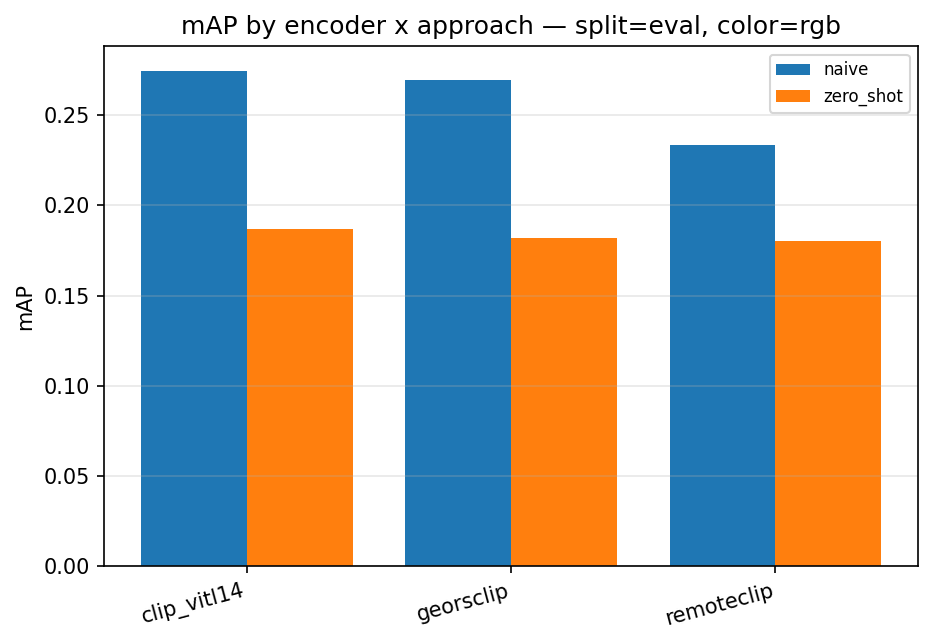
\includegraphics[width=0.8\linewidth]{map_bars__eval__rgb.png}
    \caption{QFabric change-type mAP by encoder $\times$ approach (RGB).}
    \label{fig:qfabric_eval}
\end{figure}

\subsection{QFabric PEFT --- adapter effectiveness on a second dataset}
\label{sec:qfabricpeft}

Closing the zero-shot-vs-PEFT comparison on QFabric: a stratified, crop-disjoint
train/test split (train $\leq$120 crops/class, $N$=2422 pairs; held-out test
$N$=2048), a ProjectionHead adapter trained on the train split with captions
phrased like the queries (\texttt{difference}, 40 epochs), evaluated on both
splits (Table~\ref{tab:qfabricpeft}).

\begin{table}[H]
    \centering
    \caption{QFabric PEFT (mAP). Adapter overfits train ($\approx$0.999) but on
    test sits at-or-above naive. Best per row in bold.}
    \label{tab:qfabricpeft}
    \begin{tabular}{llccc}
        \toprule
        \textbf{Encoder} & \textbf{split} & \textbf{naive} & \textbf{zero-shot} & \textbf{PEFT} \\
        \midrule
        CLIP ViT-L/14 & train & 0.278 & 0.189 & \textbf{0.998} \\
        CLIP ViT-L/14 & test  & 0.269 & 0.185 & 0.271 \\
        GeoRSCLIP     & train & 0.271 & 0.180 & \textbf{0.999} \\
        GeoRSCLIP     & test  & 0.272 & 0.181 & \textbf{0.334} \\
        RemoteCLIP    & train & 0.244 & 0.179 & \textbf{0.999} \\
        RemoteCLIP    & test  & 0.245 & 0.183 & \textbf{0.288} \\
        \bottomrule
    \end{tabular}
\end{table}

PEFT overfits train on both datasets ($\approx$0.999 here) but
generalises differently. On held-out QFabric test the adapter is at-or-above
\texttt{naive}: GeoRSCLIP $+0.062$ (0.334, the best QFabric result in this
report), RemoteCLIP $+0.043$ (0.288), CLIP neutral. This contrasts with DEN
(Section~\ref{sec:crosssplit}), where PEFT test collapsed below zero-shot
(GeoRSCLIP RGB: $0.299 \rightarrow 0.041$). The difference is what the adapter
must learn: QFabric change types are consistent visual categories (a road looks
like a road across crops), so the head learns transferable features; DEN's
directional spectral transitions are subtle and AOI-specific, so the head
memorises training-AOI statistics. PEFT's value is therefore dataset-dependent:
harmful on DEN, mildly helpful on QFabric. Both effects are small in absolute
terms, though: on QFabric a random ranker already scores mAP $\approx$0.17
(large relevant sets), so even the 0.334 PEFT is a modest lift, and DEN's best
honest figure is the cross-validated $\approx$0.20 of Section~\ref{sec:audit},
not the 0.426 single-split number. No single recipe dominates, and none is
strong.

\begin{figure}[H]
    \centering
    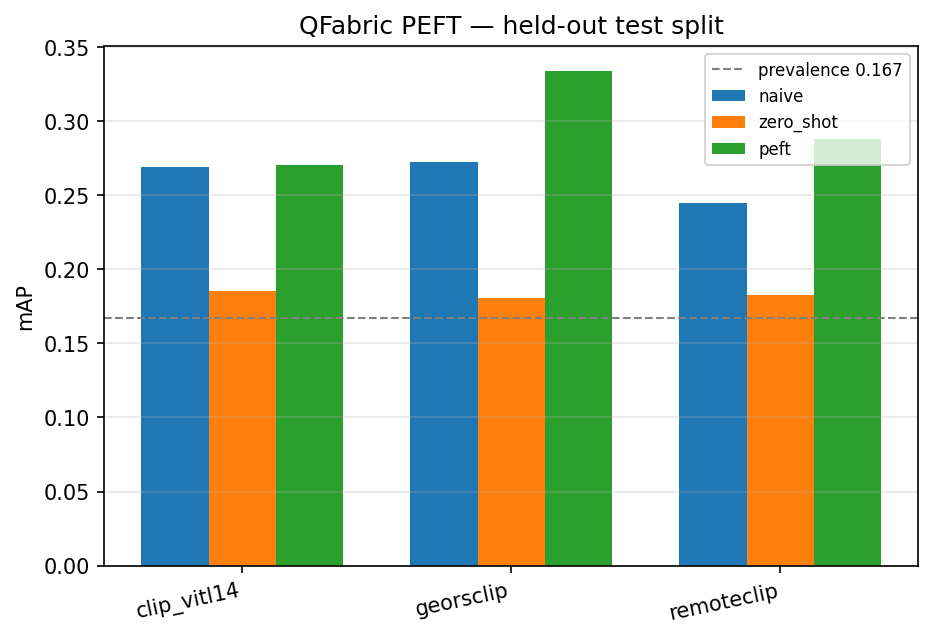
\includegraphics[width=0.8\linewidth]{qfabric_peft_test.png}
    \caption{QFabric test split: naive vs zero-shot vs PEFT.}
    \label{fig:qfabricpeft}
\end{figure}

\subsection{QFabric status-transition retrieval (RQA5) --- the regime inverts}
\label{sec:qfabricstatus}

Section~\ref{sec:qfabric} retrieved change types, a property of the after image,
for which the naive score outperformed the directional $\Delta$. QFabric also
carries a temporal task through the TEOChatlas RQA5/RTQA5 answers: the
per-timepoint development status of each region, on a nine-stage scale running
from greenland through land-cleared and construction-started to operational.
Joining each answer to its frame
(\texttt{scripts/build\_qfabric\_status\_labels.py}, dataset
\texttt{qfabric\_status}) gives every pair a status transition, and six
transition queries (\texttt{src/queries/qfabric\_status.py}, for example ``new
building construction has started'') are relevant only to pairs whose status
actually changes; stable pairs become hard negatives with the same end-state. On
a stratified subset of $\leq$120 crops per final status ($N = 4200$ pairs, frozen
encoders, RGB), Table~\ref{tab:qfabricstatus} reports mAP.

\begin{table}[H]
    \centering
    \caption{QFabric status-transition retrieval (RQA5; frozen, RGB, mAP). The
    directional zero-shot score now matches or beats naive on every encoder,
    inverting the change-type regime of Table~\ref{tab:qfabric}. Best per row in bold.}
    \label{tab:qfabricstatus}
    \begin{tabular}{lcc}
        \toprule
        \textbf{Encoder} & \textbf{naive} & \textbf{zero-shot} \\
        \midrule
        CLIP ViT-L/14 & 0.057 & \textbf{0.057} \\
        GeoRSCLIP     & 0.079 & \textbf{0.084} \\
        RemoteCLIP    & 0.064 & \textbf{0.072} \\
        \bottomrule
    \end{tabular}
\end{table}

The regime inverts: zero-shot is at least as good as naive on all three encoders
($+0.000$ CLIP, $+0.005$ GeoRSCLIP, $+0.007$ RemoteCLIP), the opposite of the
change-type result in Section~\ref{sec:qfabric}, where naive led by about 0.09.
The directional $\Delta$ is the appropriate tool for transitions, while
after-image content is the appropriate tool for types --- one dataset, two tasks,
two regimes. The edge is consistent but small, and both scores sit just above the
0.043 macro-prevalence baseline: status-transition retrieval is genuinely hard
zero-shot, with long and irregular temporal baselines and many subtle or rare
transitions. Per query the signal concentrates in the visually distinct,
well-populated transitions --- land cleared (AP 0.17) and construction started
(0.18) --- and collapses on the rare or long-range ones (demolition 0.01,
$n=32$; vacant-to-finished building 0.02, $n=64$). GeoRSCLIP is again the
strongest backbone (0.084). The broader point is that relabelling the same crops
along a temporal axis rather than a categorical one inverts which scoring
approach wins, which is direct evidence that the naive-versus-$\Delta$ trade-off
is set by task geometry rather than by the dataset.

\subsection{LEVIR-CC --- open-vocabulary retrieval on human-captioned change}
\label{sec:levircc}

The third dataset tests the engine where change is visually salient and described
in genuine human language. LEVIR-CC pairs are parsed into five open-vocabulary
change tags from their captions (Section~\ref{sec:data}) --- building, road,
demolition, vegetation, water --- and one free-text query maps to each. On the
held-out test split (1929 pairs, frozen encoders, RGB), Table~\ref{tab:levircc}
reports per-query average precision and the five-query macro. The macro
random-ranking baseline is the mean query prevalence, 0.255 (building 45.2\%,
road 42.7\%, demolition 14.8\%, vegetation 23.9\%, water 1.0\%).

\begin{table}[H]
    \centering
    \caption{LEVIR-CC open-vocabulary change retrieval (test split, 1929 pairs,
    frozen, RGB; zero-shot average precision per query, with the five-query macro
    mAP). Test positives per query in parentheses. Best per row in bold.}
    \label{tab:levircc}
    \begin{tabular}{lccc}
        \toprule
        \textbf{Query (positives)} & \textbf{GeoRSCLIP} & \textbf{CLIP ViT-L/14} & \textbf{RemoteCLIP} \\
        \midrule
        new buildings or houses (871) & 0.804 & 0.725 & \textbf{0.830} \\
        a new road or street (824)    & 0.571 & 0.631 & \textbf{0.654} \\
        buildings demolished (286)    & \textbf{0.297} & 0.138 & 0.234 \\
        trees or vegetation (462)     & 0.159 & 0.182 & \textbf{0.186} \\
        a lake, pond, or water (19)   & 0.151 & \textbf{0.221} & 0.096 \\
        \midrule
        \textbf{macro mAP (5 queries)} & 0.396 & 0.379 & \textbf{0.400} \\
        \bottomrule
    \end{tabular}
\end{table}

The five-query macro (0.38--0.40 zero-shot; naive 0.41--0.43) is held up by two
strong queries and dragged by three weak ones, so the mean is the wrong summary;
the honest reading is per-query. Building and road change --- large,
high-contrast, and described in the vocabulary the CLIP text tower was trained on
--- are retrieved strongly (buildings $\approx$0.8, roads $\approx$0.6), whereas
demolition, vegetation, and the 19-positive water class sit at or only just above
their prevalence floors. This is the same salience-proportional law the project
finds everywhere: DEN's subtle spectral transitions recover to $\approx$0.20,
QFabric construction types to $\approx$0.27, and within LEVIR-CC itself salient
construction recovers to $\approx$0.8 while subtle land-cover and sparse classes
stay near random. The RS-pre-trained encoders still gain from the directional
$\Delta$ on the strong queries (RemoteCLIP and GeoRSCLIP zero-shot beat their
naive scores on buildings) --- the same type-versus-transition split seen on
QFabric (Sections~\ref{sec:qfabric}, \ref{sec:qfabricstatus}). The lesson holds
across every dataset (DEN, QFabric, LEVIR-CC and SECOND-CC): the open-vocabulary
engine recovers the change signal in proportion to its spatial and semantic
salience --- strongly on salient construction, weakly on subtle or sparse change.

\subsection{Quantitative change localization (LEVIR-MCI)}
\label{sec:localization}

The brief asks for a heatmap highlighting the spatial region of the change. So far
that deliverable was qualitative. LEVIR-MCI (Liu et al., 2024) is a strict
superset of LEVIR-CC --- the same 1929 test pairs and captions, plus a pixel-level
change mask per pair (building, road) --- which makes the heatmap measurable. For
the two masked queries, the query-conditioned change heatmap (per-patch
$\Delta$-similarity $\cos(t,P2_p)-\cos(t,P1_p)$, the same signal as the
patch scorer of Section~\ref{sec:audit}) is scored against the mask by two metrics,
each over pairs that contain the change with at least one positive patch at grid
resolution: \emph{pointing-game} (is the highest-$\Delta$ patch a true change
patch?) and \emph{patch-AP}. Both are read against the random-patch floor (the mean
positive-patch fraction); since the patch grid differs by encoder (GeoRSCLIP
$7\times7$, the ViT-L encoders $16\times16$), each encoder is compared only to its
own floor.

\begin{table}[H]
    \centering
    \caption{LEVIR-MCI change localization (test split; pointing-game and patch-AP
    against each encoder's random-patch floor). Lift is pointing minus floor.}
    \label{tab:localization}
    \begin{tabular}{llccc}
        \toprule
        \textbf{Encoder (grid)} & \textbf{Class} & \textbf{pointing} & \textbf{floor} & \textbf{lift} \\
        \midrule
        GeoRSCLIP ($7\times7$)     & road     & 0.416 & 0.334 & \textbf{+0.082} \\
        GeoRSCLIP ($7\times7$)     & building & 0.351 & 0.378 & $-0.027$ \\
        RemoteCLIP ($16\times16$)  & road     & 0.312 & 0.208 & \textbf{+0.104} \\
        RemoteCLIP ($16\times16$)  & building & 0.257 & 0.238 & +0.019 \\
        CLIP ViT-L/14 ($16\times16$) & road     & 0.151 & 0.208 & $-0.057$ \\
        CLIP ViT-L/14 ($16\times16$) & building & 0.101 & 0.238 & $-0.137$ \\
        \bottomrule
    \end{tabular}
\end{table}

The heatmap is a weak localizer. Only road change is localized above chance, and
only by the RS-pre-trained encoders (RemoteCLIP $+0.10$, GeoRSCLIP $+0.08$
pointing-game lift); building change is not localized above its floor by any
encoder, and generic CLIP ViT-L \emph{anti-localizes} ($-0.14$ on building). This
is the spatial counterpart of the retrieval result: frozen CLIP-variant embeddings
recover change weakly, and localizing it --- a harder task than retrieving it ---
is weaker still, with only RS pre-training buying a modest road signal. The overlay
stays useful for a human in the loop, but it is not a quantitatively reliable
detector. DEN carries no instance masks, so this metric is available only on the
mask datasets (LEVIR-MCI here, SECOND-CC next).

\subsection{SECOND-CC --- open-vocabulary breadth and localisation}
\label{sec:secondcc}

LEVIR-CC's change is almost entirely building/road. SECOND-CC (Robust Change
Captioning in Remote Sensing, 2025) is the breadth counterpart: 6{,}041 pairs with
human captions \emph{and} six-class semantic maps for both phases. Seven free-text
queries cover the six SECOND classes plus road (heavily captioned, no semantic
class). Test split, 1{,}227 pairs, frozen encoders, RGB; macro random-ranking
floor 0.255.

\begin{table}[H]
    \centering
    \caption{SECOND-CC zero-shot per-query AP (test split). Buildings dominate;
    every type clears its prevalence floor but only modestly.}
    \label{tab:secondcc}
    \begin{tabular}{lccc}
        \toprule
        \textbf{Query (positives)} & \textbf{GeoRSCLIP} & \textbf{CLIP ViT-L/14} & \textbf{RemoteCLIP} \\
        \midrule
        new buildings/structures (809) & 0.698 & 0.652 & \textbf{0.702} \\
        a new road or street (460)     & \textbf{0.418} & 0.377 & 0.372 \\
        bare ground or land cleared (401) & 0.355 & \textbf{0.372} & 0.362 \\
        trees appeared/cleared (370)   & \textbf{0.341} & 0.313 & 0.334 \\
        low vegetation/grassland (311) & 0.275 & \textbf{0.280} & 0.273 \\
        a water body (167)             & \textbf{0.168} & 0.152 & 0.159 \\
        a playground/sports field (33) & 0.085 & 0.035 & \textbf{0.164} \\
        \midrule
        \textbf{macro mAP (zero-shot)} & 0.334 & 0.312 & \textbf{0.338} \\
        \textbf{macro mAP (naive)}     & \textbf{0.453} & 0.430 & 0.441 \\
        \bottomrule
    \end{tabular}
\end{table}

Across seven change types every query clears its prevalence floor --- broader
recovery than DEN, where most queries sat at random --- but only modestly: the
zero-shot macro ($\approx$0.33) is $\approx$+0.04 over the 0.255 floor, buildings
($\approx$0.70) dominate, and water/playground are weak. As on QFabric, naive
$>$ zero-shot (macro 0.45 vs 0.33): end-state appearance carries more of these
land-cover categories than the temporal $\Delta$. Localisation on the SECOND-CC
semantic masks matches the LEVIR-MCI verdict --- every reliably-sampled class sits
within $\pm$0.04 of its random-patch floor (the lone large value, playground
$+0.30$ on GeoRSCLIP, rests on 22 pairs and does not replicate). SECOND-CC thus
extends the project's central law to a wide open vocabulary: recovery scales with
the visual salience and prevalence of the change type, and is weak in absolute
terms with frozen CLIP-variant encoders.

\subsection{Error analysis --- seasonal vs permanent}
\label{sec:erroranalysis}

The benchmark reports seasonal drift@$K$ (non-relevant top-$K$ retrievals that
involve snow/ice, for permanent-change queries). On the DEN train split this is
0.00 at all $K$ for every encoder/approach --- there is essentially no
seasonal (snow/ice) class in this subset, so seasonal$\rightarrow$permanent
confusion does not arise here. The mechanism is nonetheless implemented and
exercised on the synthetic fixture, which deliberately contains a seasonal
snow-melt pair: the app flags it (``involves snow/ice --- likely
SEASONAL, not permanent'') and the benchmark would count it as drift if
mis-retrieved.

The dominant real error is not seasonal confusion but low recall from
class imbalance and weak label-derived captions (many near-stable bimonthly
pairs; agri$\leftrightarrow$wetland visually subtle). The per-query confusion
analysis (\texttt{src/error\_analysis.py}) makes this concrete: on the best test
configuration (GeoRSCLIP + NRG), the wetland queries' top-10 are dominated by
\texttt{stable} pairs (6--7 of 10), not by seasonal or wrong-transition
confusion --- i.e. the failure mode is surfacing no-change pairs
(Figure~\ref{fig:confusion}).

\begin{figure}[H]
    \centering
    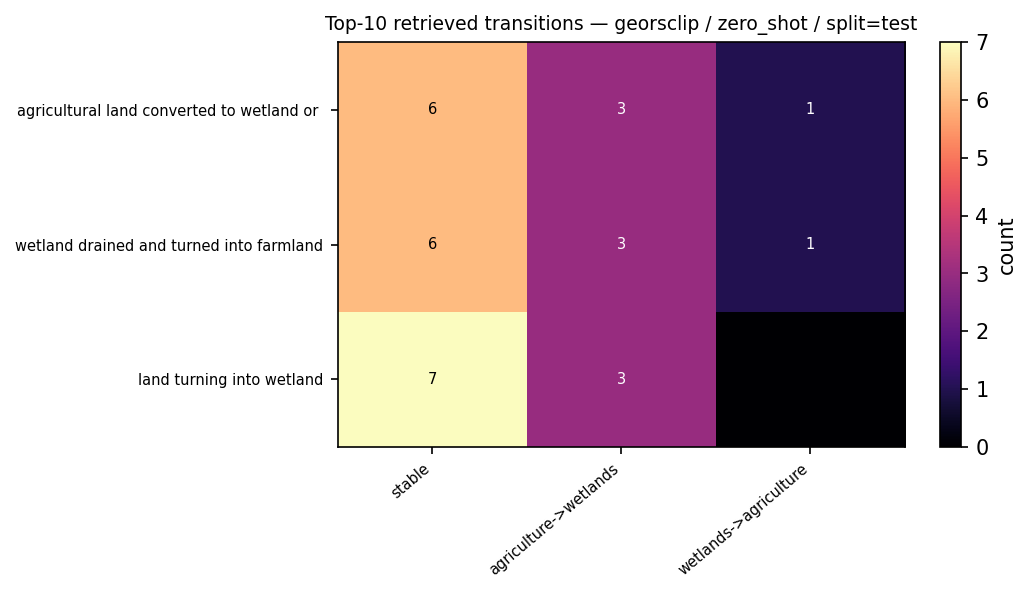
\includegraphics[width=0.8\linewidth]{confusion__georsclip__test__zero_shot.png}
    \caption{Per-query confusion (GeoRSCLIP + NRG zero-shot, test): top-$K$
    retrievals binned by actual label transition; wetland queries are dominated
    by \texttt{stable} pairs.}
    \label{fig:confusion}
\end{figure}

\subsection{Direct seasonal-robustness probe --- stable-pair $\Delta$-similarity gate}
\label{sec:seasonalgate}

Because the seasonal-drift@$K$ figure is uninformative on this subset (no snow/ice
positives, Section~\ref{sec:erroranalysis}), seasonal robustness is also probed
directly. The zero-shot score is turned into a whole-image binary gate: for a
change query $t$ and a pair's $L_2$-normalised global embeddings, the gate fires
when $\Delta = \cos(t, f_{T_2}) - \cos(t, f_{T_1}) > \tau$. On a stable pair
$f_{T_1} \approx f_{T_2}$, so $\Delta \approx 0$ for any query and every firing is
a false positive; sweeping $\tau$ over the stable subset (DEN's own
\texttt{PairLabel.stable} flag) yields a false-positive-rate curve that measures
how often seasonal or illumination drift is mistaken for change
(\texttt{src/seasonal\_gate.py}, \texttt{scripts/run\_seasonal\_gate.py}).
Table~\ref{tab:seasonalgate} reports the curve for the strongest configuration
(GeoRSCLIP, RGB, test split, 24 stable pairs).

\begin{table}[H]
    \centering
    \caption{Stable-pair false-positive rate of the $\Delta$-similarity gate
    (GeoRSCLIP, RGB, test split; 24 stable pairs, mean stable $\Delta = 0.0125$).}
    \label{tab:seasonalgate}
    \begin{tabular}{ccccc}
        \toprule
        \textbf{mean stable $\Delta$} & \textbf{FPR@0.00} & \textbf{FPR@0.02} & \textbf{FPR@0.05} & \textbf{FPR@0.10} \\
        \midrule
        0.0125 & 0.875 & 0.333 & 0.000 & 0.000 \\
        \bottomrule
    \end{tabular}
\end{table}

Stable pairs carry a near-zero mean $\Delta$-similarity (0.0125), so the
false-positive rate falls to zero once the threshold clears the noise floor, and
is already zero at $\tau = 0.05$. The high 0.875 rate at $\tau = 0$ merely
reflects that any nonzero $\Delta$ trips a zero threshold, and is not a failure
mode. The gate confirms that seasonal and illumination drift on stable pairs does
not masquerade as change once a modest threshold is applied, consistent with the
GeoRSCLIP zero-shot reading of Section~\ref{sec:nir}.


\section{Resources and operational metrics}
\label{sec:resources}

All work fits the low-compute budget of the brief: a single laptop GPU, frozen
backbones, and cached embeddings. Tables~\ref{tab:hw}--\ref{tab:timings}
summarise hardware, model sizes, disk footprint and timings.

\begin{table}[H]
    \centering
    \caption{Hardware and software.}
    \label{tab:hw}
    \begin{tabular}{ll}
        \toprule
        \textbf{Item} & \textbf{Spec} \\
        \midrule
        GPU        & NVIDIA GeForce RTX 4060 Laptop, $\sim$8\,GB VRAM \\
        Runtime    & torch 2.10.0 + CUDA (cu130); CPU fallback supported \\
        OS / Python & Windows 11 / Python 3.12.10 \\
        Optional   & free Kaggle / Colab GPU for heavier sweeps \\
        \bottomrule
    \end{tabular}
\end{table}

\begin{table}[H]
    \centering
    \caption{Model sizes. The adapter is $<$0.2\% of the backbone --- the PEFT premise.}
    \label{tab:models}
    \begin{tabular}{lrrr}
        \toprule
        \textbf{Model} & \textbf{Weights on disk} & \textbf{Params (approx)} & \textbf{Dim} \\
        \midrule
        CLIP ViT-L/14 (HF)                       & $\approx$1.71\,GB & $\approx$427\,M & 768 \\
        GeoRSCLIP (ViT-B/32 + RS5M ckpt)         & 605\,MB ckpt      & $\approx$151\,M & 512 \\
        RemoteCLIP (ViT-L/14 + ckpt)             & $\approx$1.7\,GB ckpt & $\approx$428\,M & 768 \\
        PEFT adapter (trainable part)   & 2.1--2.9\,MB      & 725{,}504 (768) / 528{,}128 (512) & --- \\
        \bottomrule
    \end{tabular}
\end{table}

\begin{table}[H]
    \centering
    \caption{Disk footprint.}
    \label{tab:disk}
    \begin{tabular}{lr}
        \toprule
        \textbf{Component} & \textbf{Size} \\
        \midrule
        DEN archive (removable after extract)        & 7.09\,GB \\
        DEN extracted                                & 9.03\,GB \\
        CLIP weights cache (in-repo, gitignored)     & $\approx$1.6\,GB \\
        HF hub cache (in-repo, gitignored)           & $\approx$2.2\,GB \\
        Embedding caches (per encoder, 605 pairs)    & CLIP 3.76\,MB, GeoRSCLIP 2.52\,MB \\
        Trained adapters                             & 2.1--2.9\,MB each \\
        Total                               & $\approx$19.5\,GB ($\approx$12.5\,GB after deleting the archive) \\
        \bottomrule
    \end{tabular}
\end{table}

\begin{table}[H]
    \centering
    \caption{Timings (RTX 4060, dedicated timed pass).}
    \label{tab:timings}
    \begin{tabular}{lr}
        \toprule
        \textbf{Operation} & \textbf{Time} \\
        \midrule
        Retrieval scoring --- numpy, 605 pairs, excl. text encode & 0.269\,ms/query \\
        End-to-end query --- CLIP text forward + scoring, 605 pairs & 10.5\,ms \\
        Embedding precompute --- CLIP L/14, $1024^2 \rightarrow 224$, GPU & 68\,ms/tile ($\approx$82\,s, one-time) \\
        PEFT training --- 605 samples, 40 epochs, adapter only, GPU & $\approx$29\,s \\
        Fast test suite --- 234 tests, mock encoders, CPU & $\approx$65\,s \\
        \bottomrule
    \end{tabular}
\end{table}


\section{Reproducibility}
\label{sec:repro}

Seeds are fixed; embeddings and adapters are cached and keyed by
(dataset, encoder, split, colour mode), with LoRA caches adding a \texttt{\_lora}
tag and cache invalidation on a pair-set change. The synthetic fixture is
regenerated automatically by the test suite. The commands below are the
reproducibility recipe used to produce the numbers in this report (a
step-by-step guide is in \texttt{README.md}).

\begin{verbatim}
pip install -e .
python -m scripts.download_den --dest data/DynamicEarthNet      # ~7 GB, one-time

# In-distribution run: train on train split, evaluate on train/val/test
python -m scripts.run_pipeline --root data/DynamicEarthNet \
    --encoder clip_vitl14 --train-split train --eval-splits train val test --epochs 40
python -m scripts.run_pipeline --root data/DynamicEarthNet \
    --encoder georsclip   --train-split train --eval-splits train val test --epochs 40
python -m scripts.run_pipeline --root data/DynamicEarthNet \
    --encoder remoteclip  --train-split train --eval-splits train val test --epochs 40

# Best generalising config: GeoRSCLIP + NRG zero-shot (no PEFT training needed)
python -m scripts.run_pipeline --root data/DynamicEarthNet \
    --encoder georsclip --color-mode nrg --eval-splits train val test --skip-train

# NDVI / NRG colour-mode ablation (zero-shot only)
python -m scripts.run_pipeline --root data/DynamicEarthNet \
    --encoder clip_vitl14 --color-mode ndvi --eval-splits train val test --skip-train
python -m scripts.run_pipeline --root data/DynamicEarthNet \
    --encoder georsclip   --color-mode ndvi --eval-splits train val test --skip-train
python -m scripts.run_pipeline --root data/DynamicEarthNet \
    --encoder remoteclip  --color-mode nrg  --eval-splits train val test --skip-train

# LoRA adapter on visual encoder (GeoRSCLIP + NRG)
python -m scripts.run_pipeline --root data/DynamicEarthNet \
    --encoder georsclip --color-mode nrg --skip-train \
    --lora --lora-epochs 20 --lora-rank 4 --lora-alpha 8 \
    --eval-splits train val test

python -m src.app --root data/DynamicEarthNet --encoder clip_vitl14 --split train  # Gradio UI

pytest -q --ignore=tests/test_text_encoder.py    # fast suite, deterministic, no network
\end{verbatim}

The figures in this report are regenerated from cached embeddings (no GPU
training) via \texttt{scripts/export\_results.py} (writes one JSON per run +
\texttt{macro\_summary.csv}) followed by \texttt{scripts/make\_figures.py} and
\texttt{scripts/make\_comparison\_figure.py}.


\section{Limitations and future work}
\label{sec:future}

Several limitations bound these results and point to future work. Supervision is
weak: captions are derived from dominant-class label flips rather than human
change descriptions, so they are noisy and coarse, and LLM-generated or
human-written change captions would be a natural improvement. Both the
ProjectionHead and LoRA adapters overfit train-AOI statistics
(Section~\ref{sec:lora}), leaving NRG zero-shot the most robust configuration;
multi-AOI held-out training or domain-randomised augmentation might address this.
Scoring still uses pooled global embeddings, and patch-level or localised change
attention (cross-attention over spatial tokens) to counter signal dilution is not
yet implemented beyond the patch top-3 scorer of Section~\ref{sec:audit}. On
QFabric both the change-type and status-transition tasks are benchmarked
(Sections~\ref{sec:qfabric}--\ref{sec:qfabricstatus}); crop-precise polygon
grounding for finer localisation remains open. fMoW is wired only at the protocol level; a
concrete loader has yet to be added. Sentinel-1/2 fusion is likewise
unimplemented: \texttt{aoi\_metadata.json} confirms 51/75 AOIs have full SAR (S1)
coverage, and feeding SAR $\Delta$-features would be a direct extension of the
NRG pattern. Re-ranking, as quantified in Section~\ref{sec:rerank}, trades mAP for
display properties rather than improving retrieval quality. Finally, all mAP
figures use LULC-derived pseudo-labels; human-annotated query relevance for a true
IR benchmark has not yet been collected.


\section{Conclusion}
\label{sec:conclusion}

The system fulfils the Case 11 brief: an open-vocabulary, frozen-backbone change
search engine with a Gradio interface, a label-grounded Recall@$K$/mAP
benchmark, seasonal-vs-permanent error analysis, and a clear zero-shot vs PEFT
comparison across three CLIP-variant encoders on Dynamic EarthNet, reported under
a strict statistical audit. Four findings emerge. First, a learned adapter shows
no out-of-distribution gain: the large in-distribution PEFT lift
($0.043 \rightarrow 0.420$, up to 0.998 on QFabric) is the adapter scored on its
own training pairs (memorisation), and under the headline GeoRSCLIP+NRG config
leakage-free cross-validated PEFT ($0.196 \pm 0.049$) merely overlaps frozen
zero-shot ($0.139 \pm 0.024$) within fold variance --- and feature-space
augmentation does not change this --- so low-compute fine-tuning is not shown to
help retrieval out-of-distribution. Second, out-of-distribution the frozen zero-shot wins, but
weakly and on an inflated headline: the widely-quoted 0.426 (GeoRSCLIP+NRG test
split) is a lucky single fold, and under 5-fold AOI cross-validation it is
$0.100 \pm 0.139$; RS pre-training and NIR false-colour help, but the absolute
signal is small. Third, the weakness is fixable evaluation plus a method ceiling,
not bad data: a relevance rule that discarded localised change starved the
benchmark, while pixel-fraction relevance restores 9/10 change-types and a
localised patch-level scorer lifts cross-validated mAP to $0.193$, making
construction change (new buildings, urban expansion) retrievable for the first
time (Section~\ref{sec:audit}); only snow is genuinely absent from the data. Fourth,
LoRA does not close the gap either (every rank/epoch overfits to test $\approx$0.07, far below frozen single-split 0.426),
consistent with the adapters-only-memorise finding.

The deliverable's value is the motivated, honestly-audited comparison, not
a single best number: spectral physics and spatial locality carry the
weak signal that exists, global embeddings and learned visual priors dilute or
memorise it, and single-split scores must be cross-validated before they are
believed. Across all four datasets the recovered signal tracks change salience:
weak on DEN's subtle spectral transitions, dataset-dependent on QFabric, strong on
LEVIR-CC's salient building/road change (per-query AP $\approx$0.6--0.8) yet
near-random on its subtle vegetation and sparse water, and --- on SECOND-CC's
seven-class open vocabulary --- above every prevalence floor but only modestly
(zero-shot macro $\approx$0.33). Localising the change (LEVIR-MCI/SECOND-CC masks)
is weaker still: the heatmap clears its random-patch floor by at most
$\approx$0.04--0.10.

\end{document}
